\documentclass{beamer}

\usepackage{multirow}
\usepackage{pgfpages}
%\setbeameroption{show notes}
\setbeameroption{show notes on second screen=right}
\mode<presentation> {
  \usetheme{Warsaw}
  \setbeamercovered{transparent}
}
\usepackage{graphicx}
\usepackage[english]{babel}
\usepackage[utf8]{inputenc}
\usepackage{times}
\usepackage[T1]{fontenc}
\usepackage{colortbl}
\usepackage{tikz}
\usepackage{pbox}
\usepackage{tcolorbox}

%\pgfdeclareimage[height=0.5cm]{le-logo}{logo-irisa}
%\logo{\pgfuseimage{le-logo}}

\setbeamertemplate{headline}{}
\setbeamertemplate{footline}[]

\AtBeginSection[]{
  \begin{frame}
  \vfill
  \centering
  \begin{beamercolorbox}[sep=8pt,center,shadow=true,rounded=true]{title}
    \usebeamerfont{title}\insertsectionhead\par%
  \end{beamercolorbox}
  \vfill
  \end{frame}
}

\setbeamertemplate{footline}[frame number]

%%%%%%%%%%%%%%%%%%%%%%%%%%%
\title[] 
{Scalable Models of Probabilistic Forecasting with Fuzzy Time Series}
%\subtitle {}

\author[] 
{Petr\^onio C\^andido de Lima e Silva\\\vspace{0.5cm} \\{\small Advisor: Frederico Gadelha Guimar\~aes} \\{\small Co-Advisor: Hossein Javedai Sadaei}}


\institute[]
{
  Machine Intelligence and Data Science (MINDS) Lab\\
  Graduate Program in Electrical Engineering - PPGEE\\
  Federal University of Minas Gerais - UFMG\\
  Belo Horizonte - MG - Brazil
}

\date[Belo Horizonte, 2019] 

\begin{document}
\newcommand{\var}{\mathcal{V}}
\newcommand{\vari}{\mathcal{V}_i}
\newcommand{\ulvar}{\tilde{A}}
\newcommand{\mlvar}{\widetilde{\mathcal{V}}_i}
\newcommand{\tlvar}{\widetilde{*\mathcal{V}}}
\newcommand{\ufset}{A_j}
\newcommand{\mfset}{A_j^{\vari}}
\newcommand{\tfset}{A_j^{*\var}}
\newcommand{\model}{\mathcal{M}}
\newcommand{\estimate}{\hat{y}(t+1)}
\newcommand{\intvl}{\mathbb{I}}
\newcommand{\interval}{\intvl = [\underline{l},\overline{u}{]}}
\newcommand{\ifts}{[\mathbb{I}]FTS}
\newcommand{\FIG}{\mathcal{FIG}}
\newcommand{\fig}{\mathcal{G}}
\newcommand{\figi}{\mathcal{G}_i}
\renewcommand{\textdegree}{$^{\circ}$}


\beamertemplatenavigationsymbolsempty
\linespread{1.0}

%%%%%%%%%%%%%%%%%%%%%%%%%%%%%%%%%%%%%%%%%%%%%%

\begin{frame}
  \titlepage
\end{frame}

\note[itemize]{
\item Good afternoon guys, it is a pleasure be here today. Thank you for attending this presentation.
\item In particular I would like to thank the board of referees and also would ask you my apologies for the inconveniences that happened 
\item My apologies for my voice, I just had a flu past week and my voice did not recovered yet.
\item Well, Let's start!
\item Today I will present the developments of my research titled "..." highlighting the most important achievements
}

%%%%%%%%%%%%%%%%%%%%%%%%%%%%%%%%%%%%%%%%%%%%%%

\begin{frame}{Schedule}
  \tableofcontents
\end{frame}

%%%%%%%%%%%%%%%%%%%%%%%%%%%%%%%%%%%%%%%%%%%%%%
%%%%%%%%%%%%%%%%%%%%%%%%%%%%%%%%%%%%%%%%%%%%%%

\section{Introduction}

%%%%%%%%%%%%%%%%%%%%%%%%%%%%%%%%%%%%%%%%%%%%%%

\begin{frame}{Introduction - Motivation}
\linespread{2}
How to represent the forecasting uncertainty in point forecasts?
\begin{itemize}
\item Uncertainties:
\begin{itemize}
\item Intrinsic / Ontological;
\item Extrinsic / Empirical;
\end{itemize}
\item Interval and Probabilistic Forecasting
\end{itemize}
\end{frame}

\note[itemize]{
\item Time Series Forecasting is one of the most important activities of the human kind
\item Forecasting is spread over several knowledge fields, engineering, economy, etc.
\item However, despite its importance, not so many people take in consideration the uncertainty inherent to the forecasting 
\item There are several kinds of uncertainties, but we will focus in the tow most important
\item Intrinsic is proper to the stochastic processes, its non-determinism, randomness, etc.
\item In the other hand, the Extrinsic uncertainty originates outside the process, is caused by instrumentation, measurement, data storage, etc
}

%%%%%%%%%%%%%%%%%%%%%%%%%%%%%%%%%%%%%%%%%%%%%%
\begin{frame}{Introduction - Uncertainty}
\linespread{2}
Why it is important to represent the uncertainty?
\begin{itemize}
\item Decision Making
\item Risk Management
\item Transparency
\item Robustness
\item Reliability
\end{itemize}
\end{frame}

\note[itemize]{
\item To know the uncertainty of the forecasts is essential for Risk Management
\item 
\item It is essential to create applications with
}

%%%%%%%%%%%%%%%%%%%%%%%%%%%%%%%%%%%%%%%%%%%%%%
\begin{frame}{Introduction - Uncertainty}
\linespread{2}
Modern Applications of Probabilistic Forecasting
\begin{itemize}
\item Dynamic and Robust Optimization
\item Intelligent Management
\item Investment Portfolio 
\item Smart Grids and Environments
\end{itemize}
\end{frame}

\note[itemize]{
\item These are some examples of modern applications of probabilistic 
\item all these applications needs of forecasting tools and also to know the uncertainty of these forecasts to improve the decision making, turning it more clever, more secure, robust
\item the key idea is: insted of to react to the uncertainty, be prepared for it
}

%%%%%%%%%%%%%%%%%%%%%%%%%%%%%%%%%%%%%%%%%%%%%%

\begin{frame}{Introduction}
\linespread{2}
Some Application Demands:
\begin{itemize}
    \item Big Data scalability;
    \item Computational performance;
    \item Auditability 
    \item Explainability 
\end{itemize}
\end{frame}

\note[itemize]{
\item One of the key points of the Big Data is velocity, therefore low cost computational methods are desired
\item European Union
\item New regulatory barriers are being imposed, especially on European Union [hics guidelines for trustworthy AI. Technical report, European Commissionon High-Level Expert Group on Artificial Intelligence (AI HLEG), 2019]
}

%%%%%%%%%%%%%%%%%%%%%%%%%%%%%%%%%%%%%%%%%%%%%%

\begin{frame}{Introduction}
\linespread{2}
Why Fuzzy Time Series?
\begin{itemize}
\item Accuracy;
\item Low computational cost;
\item Explainability;
\item Data Driven / Non Parametric;
\item Simplicity;
\item Flexibility;
\end{itemize}
\end{frame}

\note[itemize]{
\item FTS put together several features desirable for such kind of application
}

%%%%%%%%%%%%%%%%%%%%%%%%%%%%%%%%%%%%%%%%%%%%%%

\begin{frame}{Main Objectives}
\linespread{1.5}
\begin{enumerate}
\item[1] Review FTS methods and probabilistic forecasting and identify extension opportunities on known  methods;
\item[2] Propose interval and probabilistic forecasting approaches based on the Fuzzy Time Series methods;
\item[3] Improve the scalability of the proposed FTS methods in order to enable it to deal with big time series
\item[4] Propose a method for Hyperparameter Optimization - DEHO;
\item[5] Extend the proposed methods to enable multivariate time series;
\end{enumerate}
\end{frame}

\note[itemize]{
\item The objectives sought during this research
}

%%%%%%%%%%%%%%%%%%%%%%%%%%%%%%%%%%%%%%%%%%%%%%
%%%%%%%%%%%%%%%%%%%%%%%%%%%%%%%%%%%%%%%%%%%%%%

\section{Fuzzy Time Series}

\note[itemize]{
\item We start by defining what are the Fuzzy Time Series 
}

%%%%%%%%%%%%%%%%%%%%%%%%%%%%%%%%%%%%%%%%%%%%%%
\begin{frame}{Definitions and notations}
\begin{table}[]
    \centering
    \begin{tabular}{|c|m{7cm}|} \hline
        $Y \in \mathbb{R}^1$ &  the univariate time series \\ \hline
        $y(t) \in Y$ & an individual instance of $Y$ \\ \hline
        $T \in \mathbb{R}^1$ & the total length of $Y$ \\ \hline
        $t \in T$ & the time index \\ \hline
        $U$ & the Universe of Discourse of $Y$ \\ \hline
        $\ulvar$ & the linguistic variable, the group of fuzzy sets created for $Y$ \\ \hline
        $\ufset \in \ulvar$ & the individual fuzzy sets in $\lvar$ \\ \hline
        $F$ & the fuzzyfied time series \\ \hline
        $f(t) \in F$ & an individual instance of $F$ \\ \hline
    \end{tabular}
\end{table}
\end{frame}

\note[itemize]{
\item This symbols are used hereinafter to define some common time series and FTS concepts
\item CAPITAL letters usually refer to sets 
\item LOWER letters usually refer to instances
}

%%%%%%%%%%%%%%%%%%%%%%%%%%%%%%%%%%%%%%%%%%%%%%

\begin{frame}{Fuzzy Time Series}
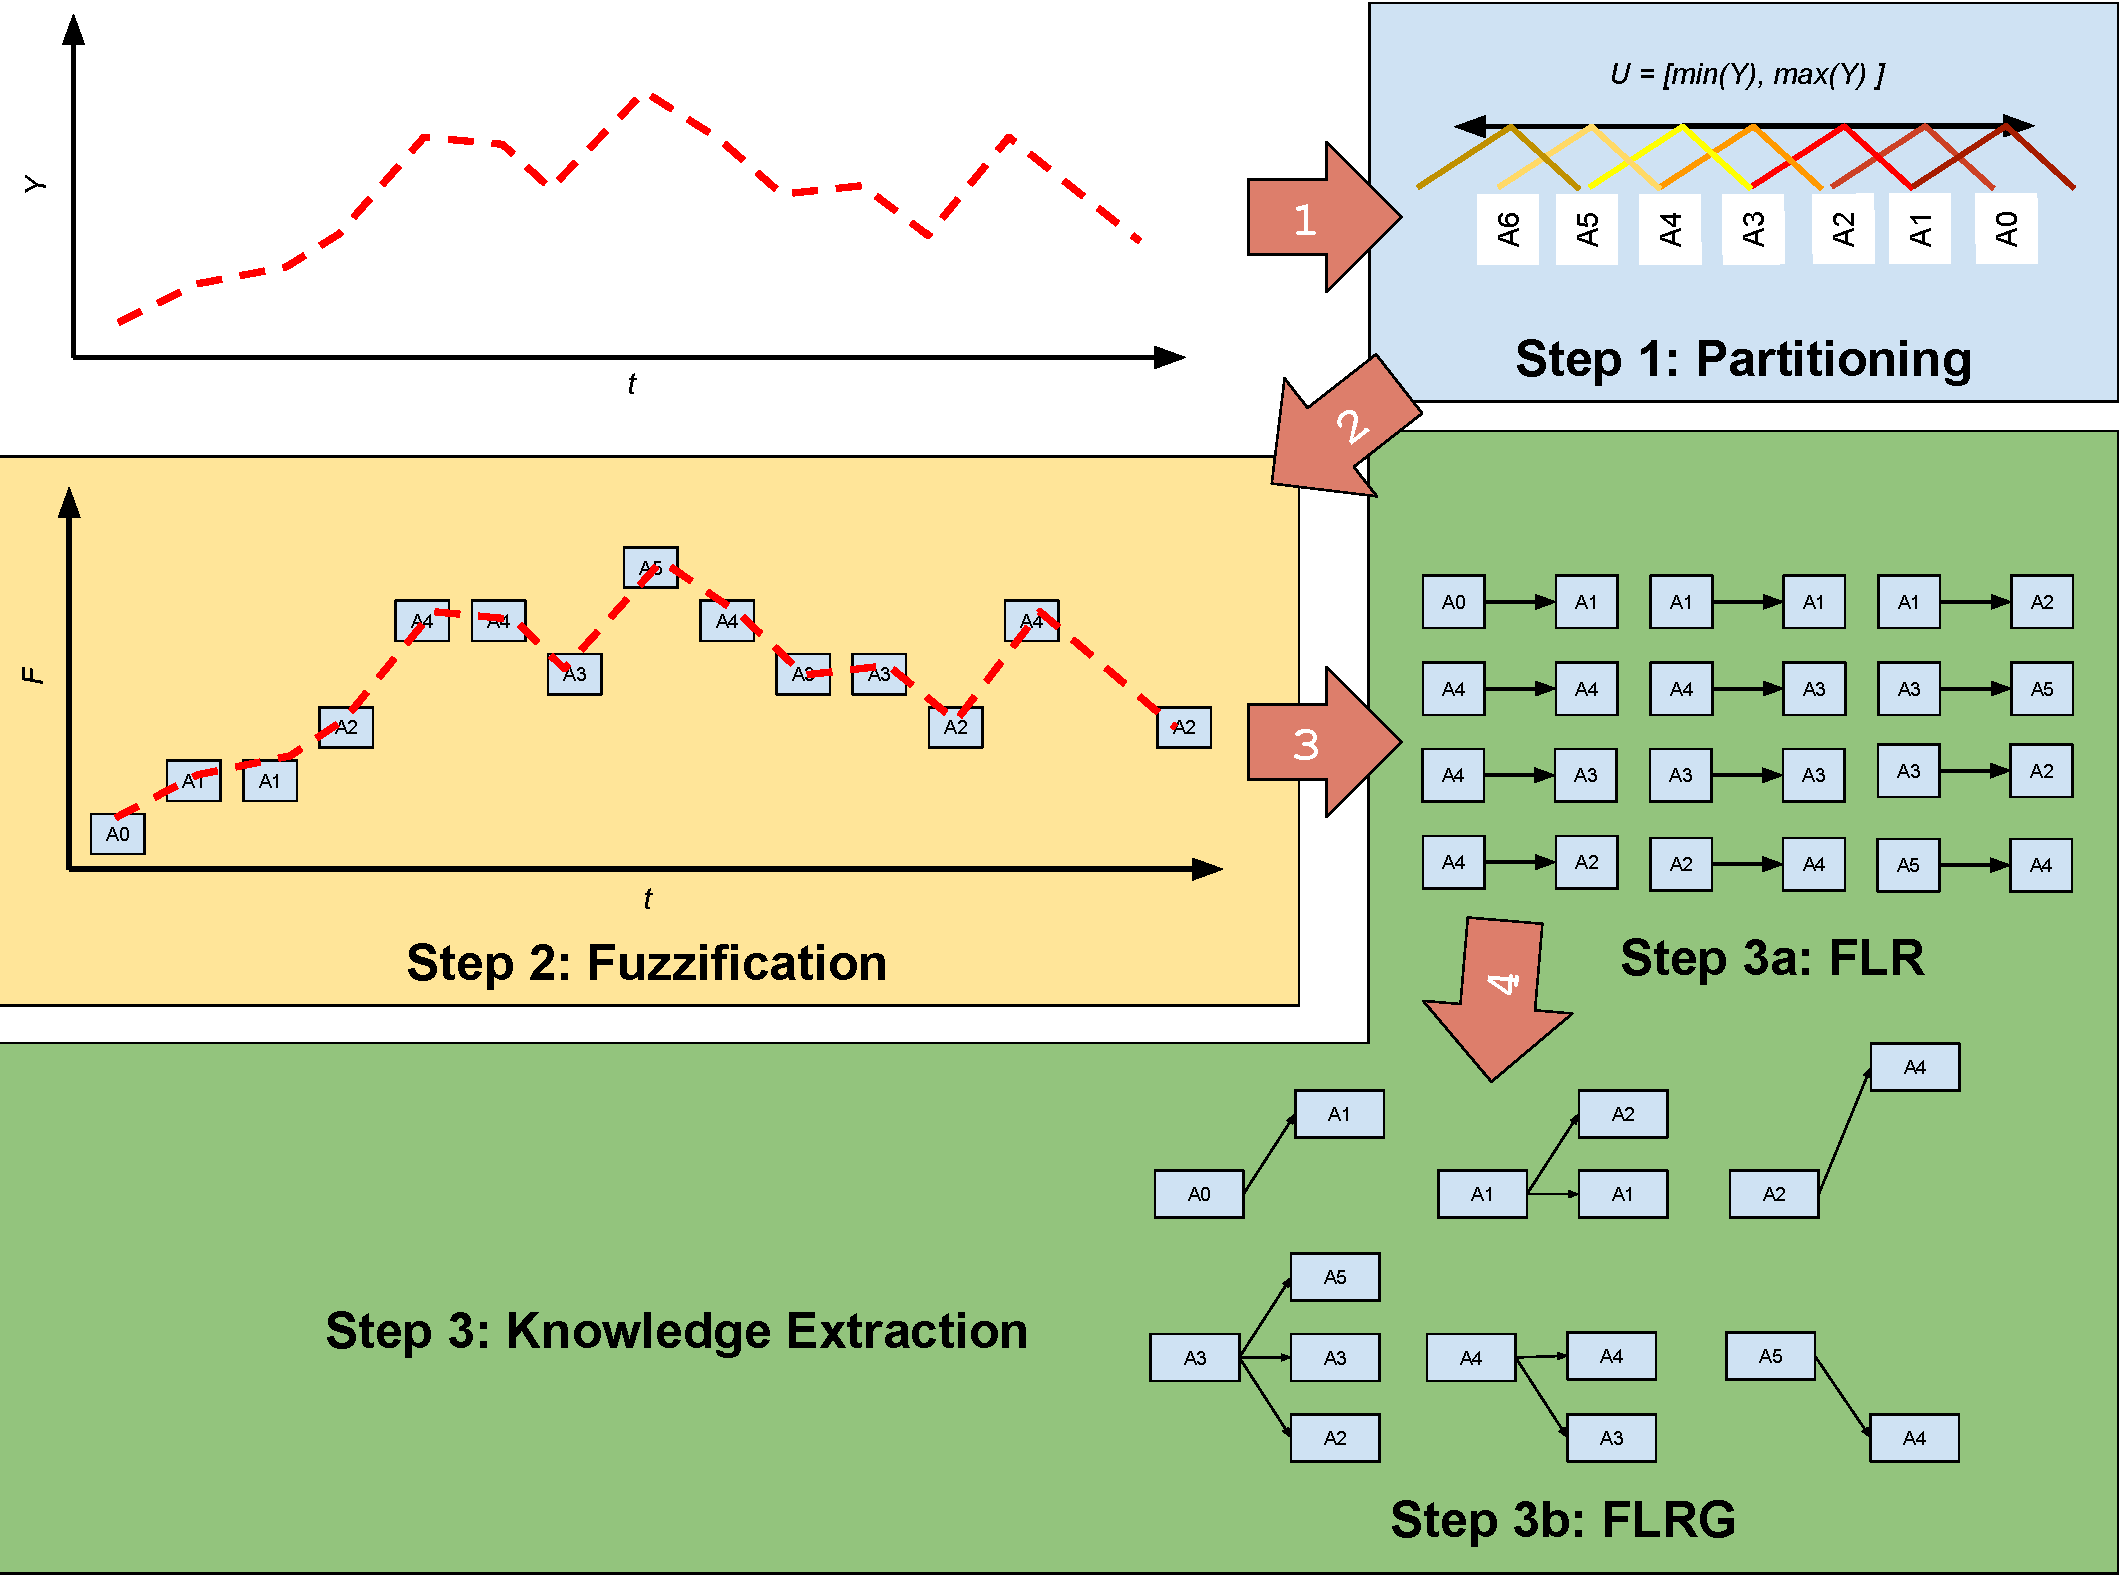
\includegraphics[width=\textwidth,height=8cm]{figures/fts_simplified.pdf}
\end{frame}

\note[itemize]{
\item The general FTS approach is simple and it is based on these main stages
\item The first FTS method were published in 1993 by Song and Chissom and used matrices to represent the temporal transitions between the fuzzy sets
\item Chen published in 1996 an improvement of the Song and Chissom method, which is based on rules - the FLRG
}


%%%%%%%%%%%%%%%%%%%%%%%%%%%%%%%%%%%%%%%%%%%%%%

\begin{frame}{Fuzzy Time Series - Training Procedure}
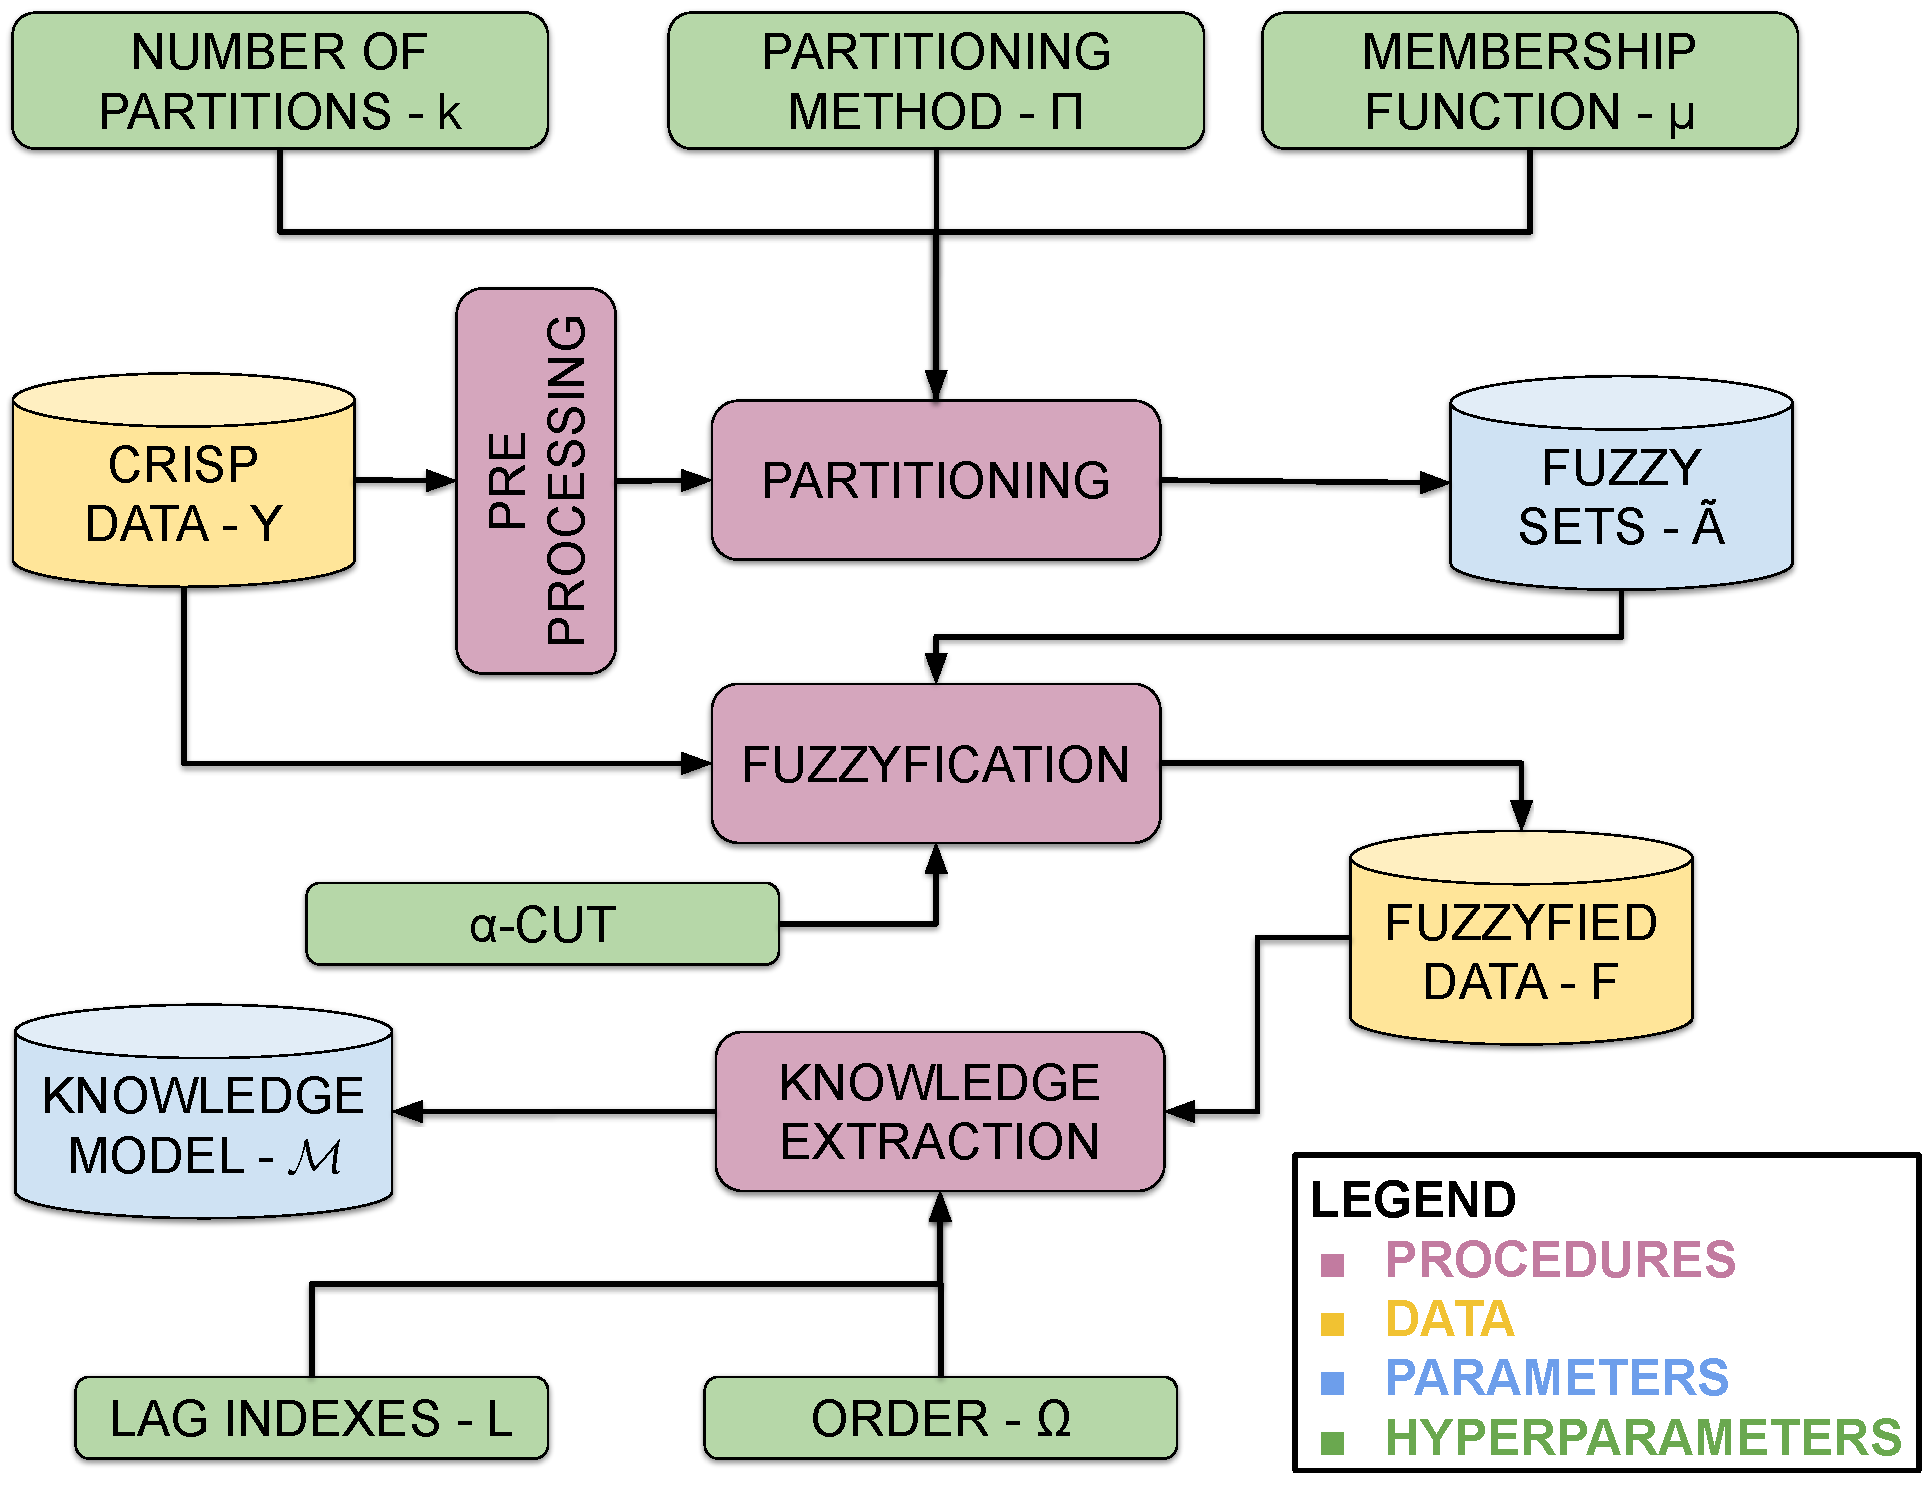
\includegraphics[width=\textwidth,height=8cm]{figures/fts_training.pdf}
\end{frame}

\note[itemize]{
\item Over the years several other improvements were proposed, extending FTS methods to a more complex framework
\item This figure represents a consensus method based on the most important contributions of the last years.
}

%%%%%%%%%%%%%%%%%%%%%%%%%%%%%%%%%%%%%%%%%%%%%%
\begin{frame}{HOFTS and WHOFTS Model Parameters}
\scriptsize
\begin{center}
$LHS \rightarrow RHS$

IF $F(t)$ is $A_i$ THEN $F(t+1)$ WILL BE $A_j$ OR $A_k$ ...    
\end{center}

\begin{columns}
\column{0.5\textwidth}
\begin{block}{Example FLRG set ($k=6$, $\Omega=1$)}
$$
\begin{array}{rcl}
A_1  & \rightarrow &  A_1 \\
A_2  & \rightarrow &  A_2,\  A_3 \\
A_3  & \rightarrow &  A_3,\  A_4 \\
A_4  & \rightarrow &  A_3,\  A_4,\\
& & \  A_5 \\
A_5  & \rightarrow &  A_6 \\
A_6  & \rightarrow &  A_5,\  A_6 \\
\end{array}
$$
\end{block}
\begin{block}{HOFTS Defuzzyfication}
$$
\begin{array}{rcl}
    mp_j & = & \displaystyle |RHS|^{-1}\sum_{i \in RHS} w_i \cdot c_i  \\
     \\
     \hat{y}(t+1) & = & \displaystyle \frac{\sum_{j \in K} \mu_j\cdot mp_j}{\sum_{j \in K} \mu_j}
\end{array}
$$
\end{block}
\column{0.5\textwidth}
\begin{block}{Example Weighted FLRG Set ($k=6$, $\Omega=1$)}
$$
\begin{array}{rcl}
A_1  & \rightarrow &  (1.0)\; A_1 \\
A_2  & \rightarrow &  (0.667)\; A_2,\  (0.333)\; A_3 \\
A_3  & \rightarrow &  (0.75)\; A_3,\  (0.25)\; A_4 \\
A_4  & \rightarrow &  (0.167)\; A_3,\  (0.667)\; A_4,\\
& & \  (0.167)\; A_5 \\
A_5  & \rightarrow &  (1.0)\; A_6 \\
A_6  & \rightarrow &  (0.333)\; A_5,\  (0.667)\; A_6 \\
\end{array}
$$
\end{block}
\begin{block}{WHOFTS Defuzzyfication}
$$
\begin{array}{rcl}
     mp_j & = & \sum_{i \in RHS} w_i \cdot c_i  \\
     \\
     \displaystyle \hat{y}(t+1) & = &  \displaystyle \frac{\sum_{j \in K} \mu_j \cdot mp_j}{\sum_{j \in K} \mu_j}
\end{array}
$$
\end{block}
\end{columns}
\end{frame}

\note[itemize]{
\item The rule-based knowledge representation is easy to read and explain
\item Each rule is composed by a precedent (LHS), and the consequent (RHS) and can be interpreted as...
\item These figures show the difference between HOFTS and WHOFTS rules and their defuzzyfication processes.
\item Each weight is the normalized frequency of each fuzzy set in the consequent
}

%%%%%%%%%%%%%%%%%%%%%%%%%%%%%%%%%%%%%%%%%%%%%%

\begin{frame}{Fuzzy Time Series - Forecasting Procedure}
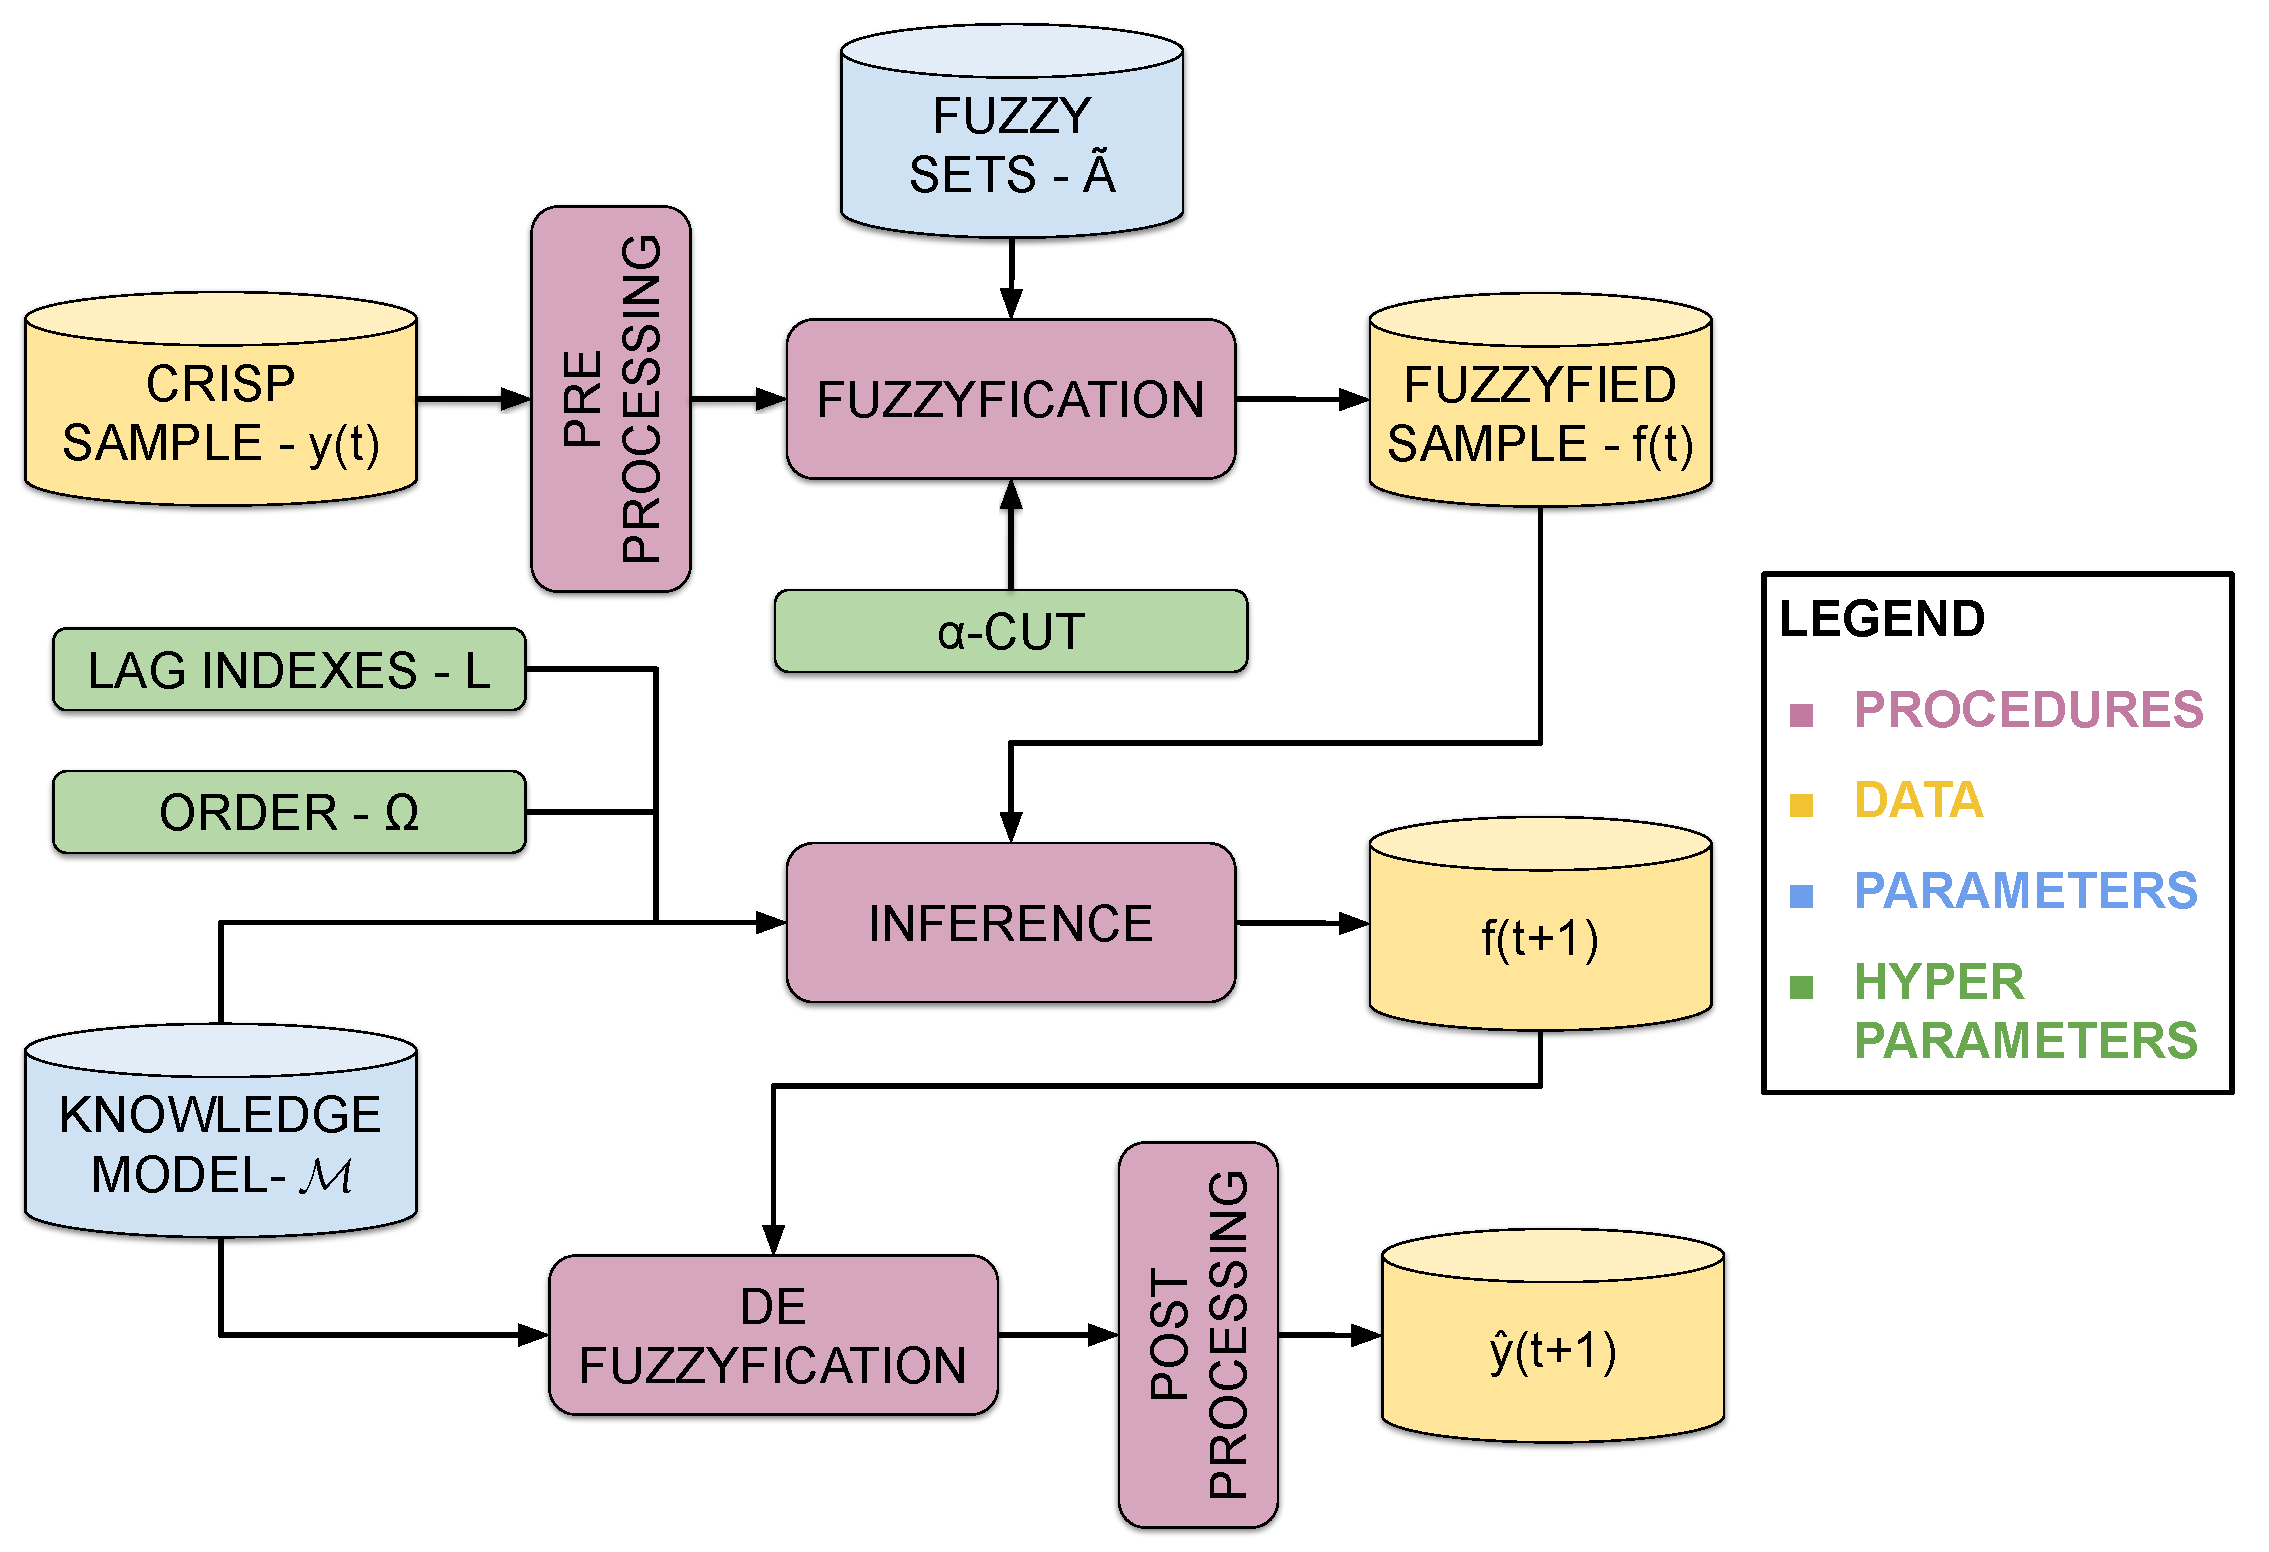
\includegraphics[width=\textwidth,height=8cm]{figures/fts_forecasting.pdf}
\end{frame}


%%%%%%%%%%%%%%%%%%%%%%%%%%%%%%%%%%%%%%%%%%%%%%

\begin{frame}{Fuzzy Time Series Models}
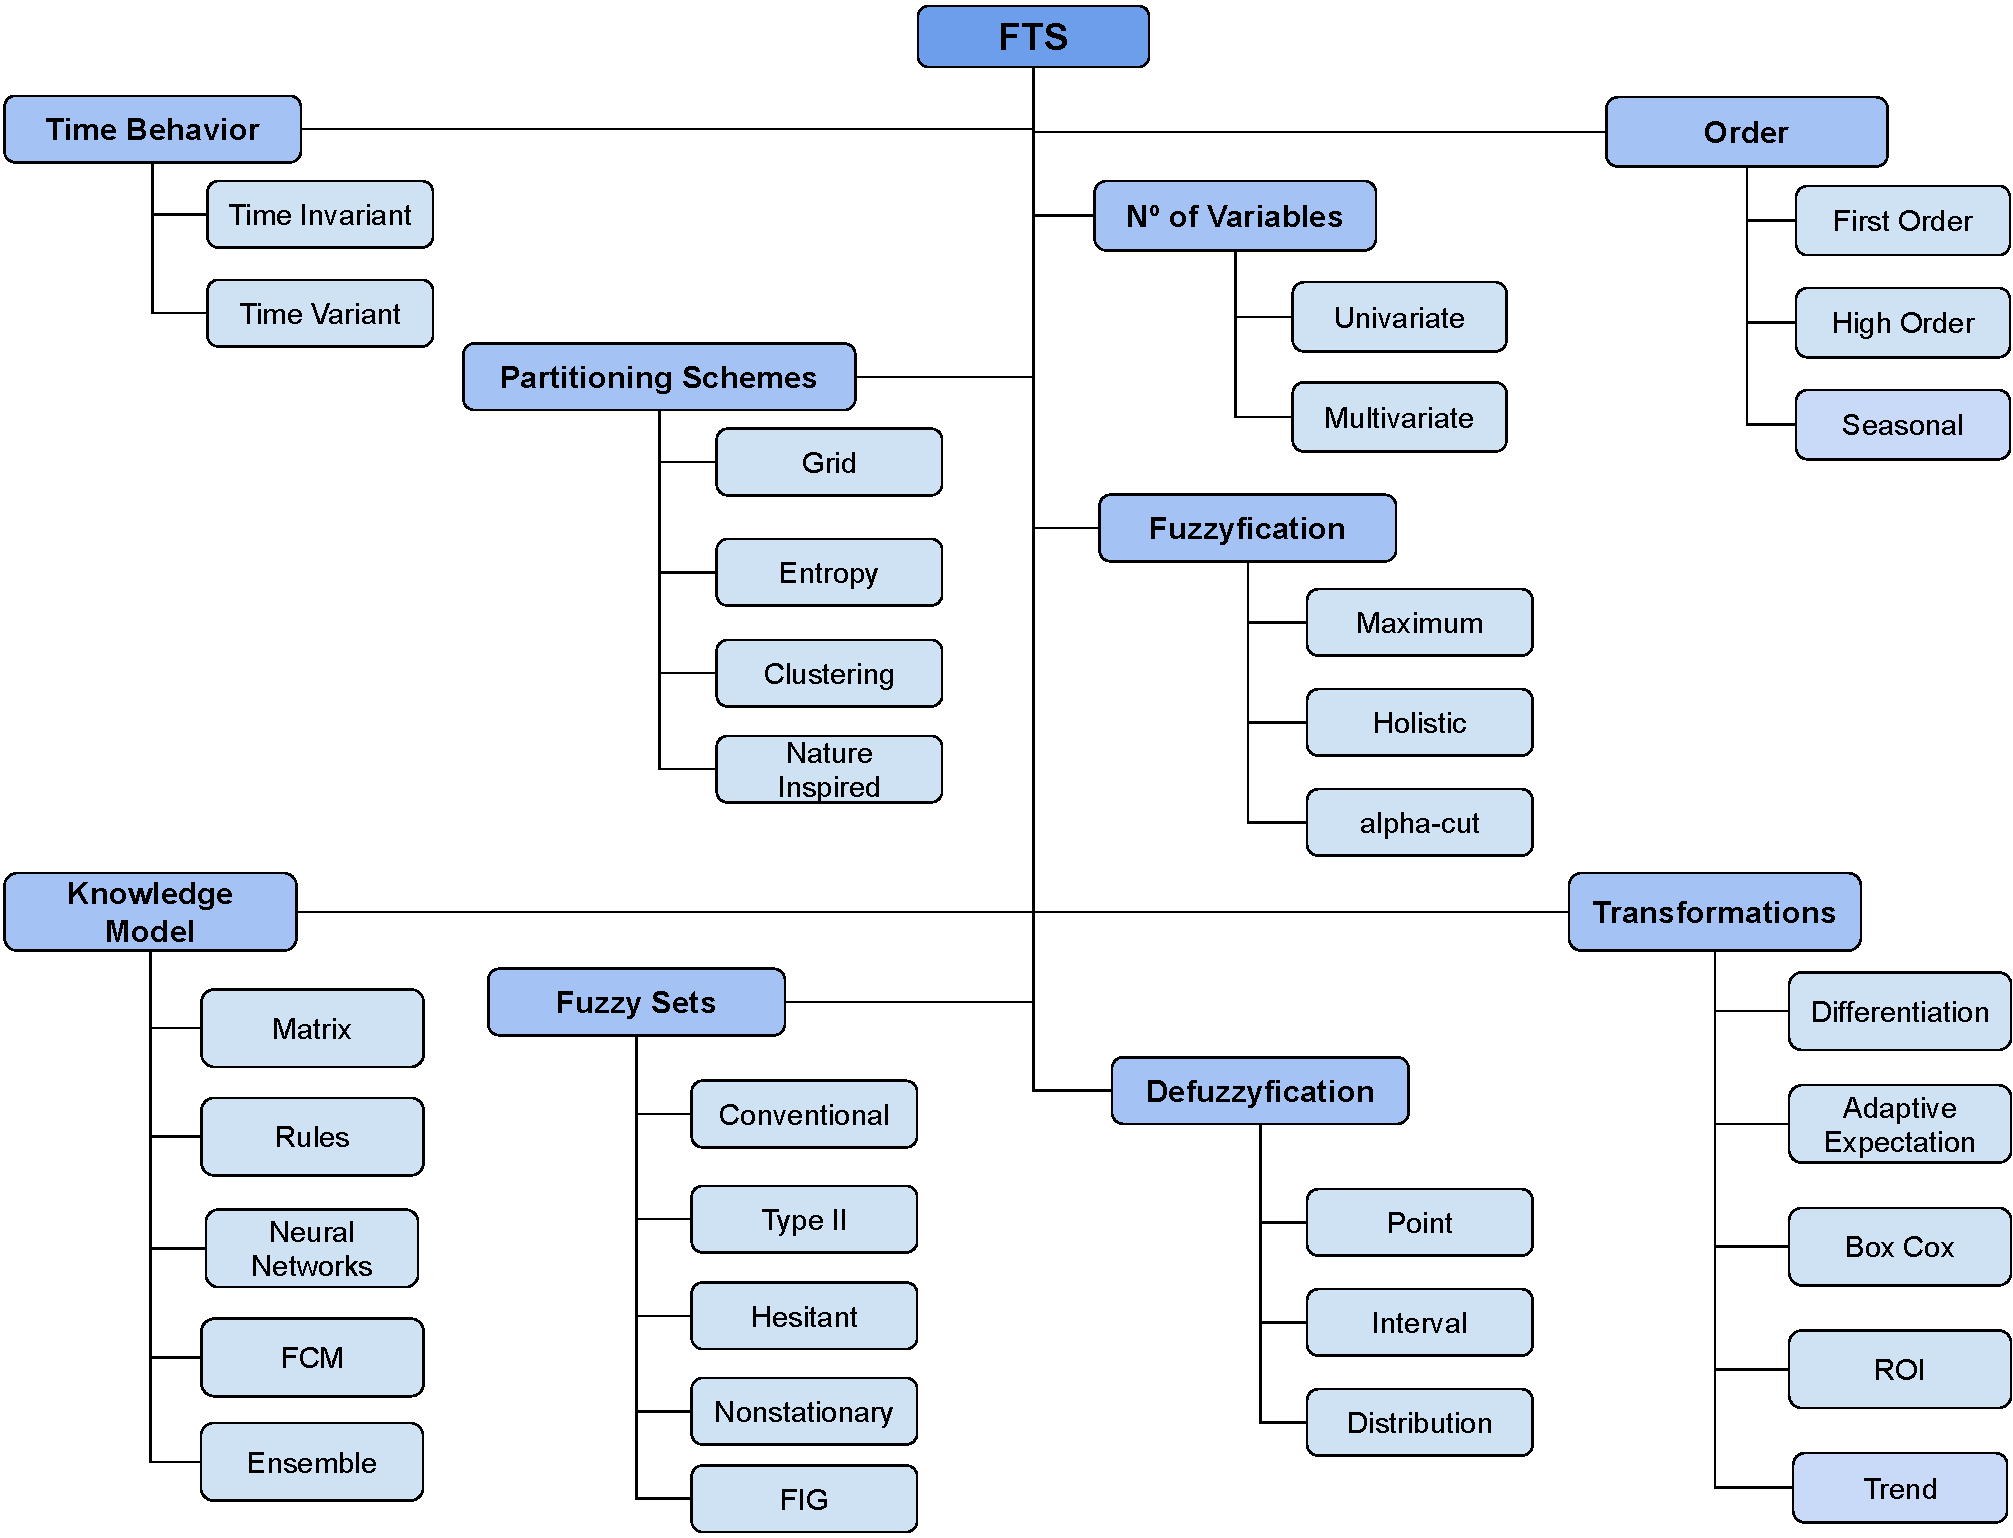
\includegraphics[width=\textwidth,height=8cm]{figures/fts_taxonomy.pdf}
\end{frame}

\note[itemize]{
\item CUSTOMIZABLE
\item In this figure we can see a little sample of the FTS flexibility
\item There is a wide variety of components for FTS 
\item The most important parameters are the Time Behavior, Order and partitioning scheme
}

%%%%%%%%%%%%%%%%%%%%%%%%%%%%%%%%%%%%%%%%%%%%%%

\begin{frame}{Fuzzy Time Series Models - Scope}
\begin{table}[]
    \centering
    \begin{tabular}{|c|c|} \hline
         \textbf{Time Behavior} & Time Invariant  \\ \hline
         \textbf{Partitioning Scheme} & Grid  \\ \hline
         \textbf{Order} & High Order  \\ \hline
         \textbf{Fuzzyfication} & Holistic  \\ \hline
         \textbf{Knowledge Mode} & Rule Based  \\ \hline
         \textbf{Fuzzy Sets} & Conventional  \\ \hline
         \textbf{Transformations} & None  \\ \hline
    \end{tabular}
    \caption{FTS scopes of this research}
    %\label{tab:my_label}
\end{table}
\begin{itemize}
    \item Consensus methods:
    \begin{enumerate}
        \item High Order Fuzzy Time Series (HOFTS)
        \item Weighted High Order Fuzzy Time Series (WHOFTS)
    \end{enumerate}
\end{itemize}
\end{frame}

\note[itemize]{
\linespread{2}
\item With such variety of components we had to impose limits in our research scope, or the research would be endless
\item This table show some imposed constraints in the FTS components that make the research scope more strict
\item Instead of reference several methods, each one with few improvements we propose the consensus methods to simplify the method comparations
\item The consensus methods were proposed as an aggregation of the most important contributions for the FTS in the last years 
}


%%%%%%%%%%%%%%%%%%%%%%%%%%%%%%%%%%%%%%%%%%%%%%

\begin{frame}{HOFTS and WHOFTS Hyperparameters}
\small
\begin{table}[]
    \centering
    \begin{tabular}{|c|l|c|} \hline
        \textbf{Alias} & \textbf{Parameter} & \textbf{Type} \\ \hline
         $k$ & Number of partitions & $\mathbb{N}^+$  \\ \hline
         $\Omega$ & Order & $\mathbb{N}^+ \geq 1$  \\ \hline
         $\Pi$ & Partitioning scheme & $\Pi: Y \rightarrow \ulvar$  \\ \hline
         $L$ & Lag indexes & $\mathbb{N}^+$  \\ \hline
         $\mu$ & Membership function & $\mu: U \rightarrow [0,1]$  \\\hline
         $\alpha$ & $\alpha$-cut & $[0,1]$ \\ \hline
    \end{tabular}
    \caption{HOFTS and WHOFTS hyperparameters}
    \label{tab:hyperparameters}
\end{table}
\end{frame}

\note[itemize]{
\item 
}



%%%%%%%%%%%%%%%%%%%%%%%%%%%%%%%%%%%%%%%%%%%%%%

\begin{frame}{Fuzzy Time Series}
\linespread{2}
\begin{itemize}
\item How to represent the uncertainty of FTS forecasts?
\begin{itemize}
    \item No interval or probabilistic methods!
\end{itemize}
\item How the uncertainty grows as the forecasting horizon increases?
\end{itemize}
\end{frame}

\note[itemize]{
\item Our experiments showed that FTS has accuracy comparable with the most known forecasting methods.
\item The main drawback of the FTS until this work is that they just forecast points;
}

%%%%%%%%%%%%%%%%%%%%%%%%%%%%%%%%%%%%%%%%%%%%%%
%%%%%%%%%%%%%%%%%%%%%%%%%%%%%%%%%%%%%%%%%%%%%%

\section{Interval Forecasting}

%%%%%%%%%%%%%%%%%%%%%%%%%%%%%%%%%%%%%%%%%%%%%%
\begin{frame}{Interval Forecasting}
\begin{itemize}
\item Prediction Intervals - \cite{Chatfield1993}
$$
\interval \qquad P(\underline{l} \leq y(t+1) \leq \overline{u}) = 1 - \alpha \qquad \alpha \in (0,1)
$$
\item Mean-Variance Models - \cite{Chatfield2001}
\begin{equation}
    \begin{array}{rcl}
        \intvl & = & [\underline{\mu - z_{\alpha/2}\sigma_\epsilon}\ ,\ \overline{\mu + z_{\alpha/2}\sigma_\epsilon}] \\
        & & \\
         \mu &=& \mathbb{E}[Y_{t+1}|Y_t,Y_{t-1},...] \\
         \sigma_\epsilon & = & \sqrt{VAR[\epsilon]} \qquad
         \epsilon  \sim  \mathcal{N}(0,1) \\
         z_{\alpha/2} & = & \Phi((1- \alpha)/2)
    \end{array}
\end{equation}
\end{itemize}
\end{frame}

\note[itemize]{
\item Prediction intervals are composed by a lower and upper bounds
\item the PI is expected to contain the future value with a confidence level alpha
\item Mean variance depends on the residual normality, z is the standard score $\ = \frac{x - \mu}{\sigma}$ function
\item $\Phi$ is the cumulative standard normal distribution
}

%%%%%%%%%%%%%%%%%%%%%%%%%%%%%%%%%%%%%%%%%%%%%%
\begin{frame}{Interval Forecasting}
\linespread{1.5}
\begin{itemize}
\item Inter-quantile Interval
$$
\begin{array}{rcl}
         \intvl & = & [\underline{Q(\alpha/2)}, \overline{Q(1-\alpha/2)}]  \\
        Q(\tau) & = & \arg\min_x\{ x \in U \ |\ \tau < F(x) \} \\
        \tau & \in & (0,1)
    \end{array}
$$
\item Quantile Auto-Regression - QAR(p)
\begin{itemize}
\item \cite{Koenker2006}, \cite{Takeuchi2006}, \cite{Hansen2006}
\end{itemize}
\end{itemize}
$$
    \begin{array}{rcl}
        Q_{y(t)}(\tau | y(t-1),\ldots) & = & \min_\theta \sum_{i=1}^n \rho_\tau (y(t) - y(i)\theta \\
        \rho_\tau(u) & = & u(\tau - \mathbf{1}(u < 0)) 
    \end{array}
$$
\end{frame}

\note[itemize]{
\item The interquantile interval can be defined with a confidence level $\alpha$
\item The quantile function uses the cumulative distribution function to find the value that best represent the quantile
\item When CDF is not available it is necessary to minimize the Pinball Loss Function to find the quantile
\item QAR is an autoregressive model that fits parameters that infer the best value for a given quantile $\tau$
}

%%%%%%%%%%%%%%%%%%%%%%%%%%%%%%%%%%%%%%%%%%%%%%
\begin{frame}{Interval Forecasting - Many Steps Ahead}
\linespread{2}
\begin{itemize}
\item $H \in \mathbb{N}^+$: the forecasting horizon
\item How uncertainty grows as $H \rightarrow \infty$ ?
\item Mean-Variance
\begin{itemize}
\item $\sigma_\epsilon^h = (1 + h\beta)\sigma_\epsilon^1$, for some smoothing value $\beta \in (0,1)$
\end{itemize}
\item Quantile Auto-Regression - QAR(p)
\begin{itemize}
\item A particular model must be fitted for each $h \in H$
\end{itemize}
\end{itemize}
\end{frame}

\note[itemize]{
\item 
}

%%%%%%%%%%%%%%%%%%%%%%%%%%%%%%%%%%%%%%%%%%%%%%

\begin{frame}{Evaluating Interval Forecasts}
\linespread{2}
\begin{itemize}
\item Coverage, Sharpness, Resolution, Pinball Score
\item Winkler Score
$$
WS(\alpha, y(t), \intvl(t)) = \left\{ \begin{array}{ccl}
\delta & if & \underline{l} \leq y \leq \overline{u} \\
\delta + 2(\underline{l} - y)/\alpha & if & y < \underline{l}  \\
\delta + 2(y - \overline{u})/\alpha & if & \overline{u} < y   
\end{array} \right.
$$
\end{itemize}
\end{frame}

\note[itemize]{
\item Intervals can be evaluated using several perspectives, as its hit rate (cov), average range (shp), range variation (res) or proximity to an especific quantile (ps)
\item Winkler Score try to condensate all these measures
\item In the equation is possible to see all these components
}

%%%%%%%%%%%%%%%%%%%%%%%%%%%%%%%%%%%%%%%%%%%%%%

%%%%%%%%%%%%%%%%%%%%%%%%%%%%%%%%%%%%%%%%%%%%%%

\begin{frame}{Interval Fuzzy Time Series  - $[\mathbb{I}]$FTS}
\linespread{2}
\begin{itemize}
\item Represents the total fuzzy uncertainty contained in the consequent of the fuzzy rules
\item The interval contains minimum and maximum possible values;
\item Can be adapted to work with all rule-based FTS methods;
\item Only changes the Forecasting Procedure;
\end{itemize}
\end{frame}

\note[itemize]{
\item To initially bring the FTS to the interval forecasting field we propose the IFTS method
\item The FTS methods use FLRG to forecast and each FLRG can have many RHS sets, the real value can be at any point inside that fuzzy sets
}

%%%%%%%%%%%%%%%%%%%%%%%%%%%%%%%%%%%%%%%%%%%%%%

\begin{frame}{$[\mathbb{I}]$FTS Deffuzification procedure}
\linespread{1.5}
\begin{itemize}
\item Each chosen FLRG will generate an interval 
\item Each interval is composed by the RHS fuzzy set bounds
$$
\begin{array}{lcr}
\mathbb{I}^i_{min} & = & \min( \underline{A_1}, ..., \underline{A_k} ) \\
& & \\
\mathbb{I}^i_{max} & = & \max( \overline{A_1}, ..., \overline{A_k} ) \\ 
& & A_1, ..., A_k \in RHS 
\end{array}
$$
\item The final forecast is the weighted sum of the intervals by the membership degree of the LHS
$$
\mathbb{I}(t+1) = \frac{\sum_{j \in A} \mu_i \mathbb{I}^j}{\sum_{j \in A} \mu_j} = \frac{\sum_{j \in A} [\mu_j\underline{\mathbb{I}^j_{min}} , \mu_j\overline{\mathbb{I}^j_{max}}] }{\sum_{j \in A} \mu_j}
\label{eqn:ifts}
$$
\end{itemize}
\end{frame}

\note[itemize]{
\item 
}


%%%%%%%%%%%%%%%%%%%%%%%%%%%%%%%%%%%%%%%%%%%%%%

\begin{frame}{Weighted $[\mathbb{I}]$FTS}
\begin{itemize}
    \item The bounds of the intervals are the weighted sum of the bounds of the RHS fuzzy sets
    $$
\begin{array}{ccc}
\intvl_{min} & = & \sum_{j \in RHS} w_j \cdot \underline{\ufset} \\
& & \\
\intvl_{max} & = & \sum_{j \in RHS} w_j \cdot \overline{\ufset}
\end{array}
\label{eqn:weighted_iminimax}
$$
\item Final forecast
$$
\mathbb{I}(t+1) = \frac{\sum_{j \in A} \mu_i \mathbb{I}^j}{\sum_{j \in A} \mu_j} = \frac{\sum_{j \in A} [\mu_j\underline{\mathbb{I}^j_{min}} , \mu_j\overline{\mathbb{I}^j_{max}}] }{\sum_{j \in A} \mu_j}
\label{eqn:ifts}
$$
\end{itemize}
\end{frame}


\note[itemize]{
\item The step 4 mix all intervals of the chosen FLRG's weighted by their membership values
\item 
}

%%%%%%%%%%%%%%%%%%%%%%%%%%%%%%%%%%%%%%%%%%%%%%
\begin{frame}{PWFTS Forecasting Sample}
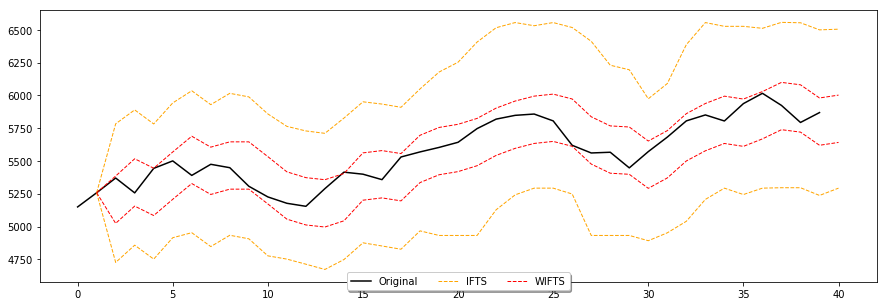
\includegraphics[width=\textwidth,height=5cm]{figures/ifts_sample_onestep.png}
\end{frame}

\note[itemize]{
\item This figure compares the intervals generated by IFTS and WIFTS methods for one step ahead forecasting
\item WIFTS is sharper but with less coverage
\item IFTS is less sharp but with high coverage
\item the length of the intervals is directly impacted by the number of fuzzy sets
}

%%%%%%%%%%%%%%%%%%%%%%%%%%%%%%%%%%%%%%%%%%%%%%
\begin{frame}{$\ifts$ Many Steps Ahead}
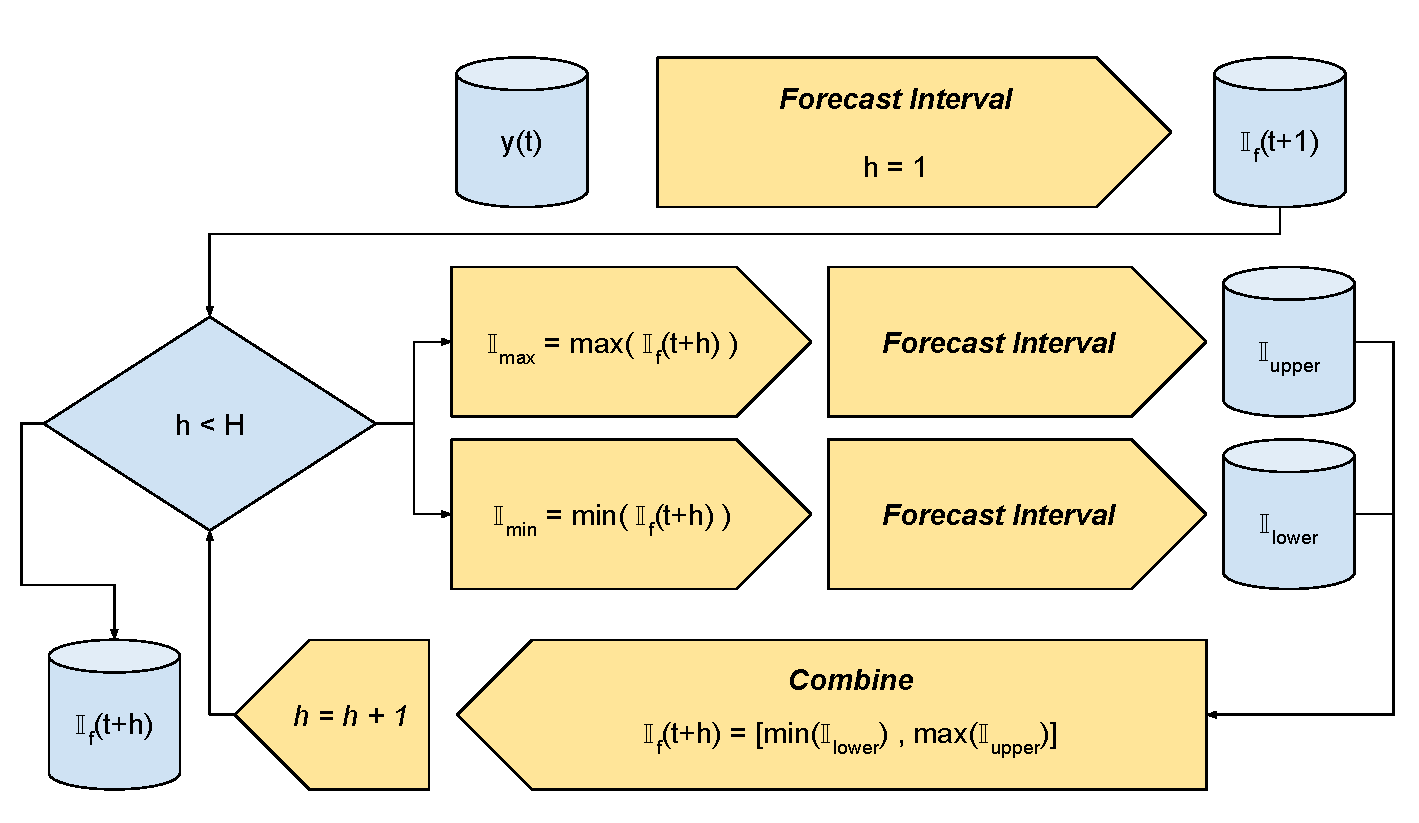
\includegraphics[width=\textwidth]{figures/ifts_many_steps.pdf}
\end{frame}

\note[itemize]{
\item This diagram show how the many steps ahead intervals are calculated
\item The approach always consider the extremum values, or the worst cases scenarios - if you consider that the best case is when real value fall in the middle of the interval
}

%%%%%%%%%%%%%%%%%%%%%%%%%%%%%%%%%%%%%%%%%%%%%%
\begin{frame}{$\ifts$ Many Steps Ahead}
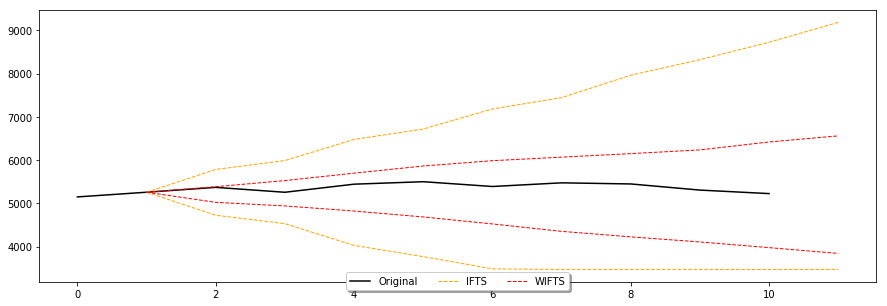
\includegraphics[width=\textwidth,height=6cm]{figures/ifts_sample_manystep.png}
\end{frame}

\note[itemize]{
\item This figure shows a sample of the 10 steps ahead interval forecasting
\item This figure reveals how the uncertainty of IFTS propagates over the forecasting horizon
\item The main drawback is that the intervals often reach the bounds of the UoD
}

%%%%%%%%%%%%%%%%%%%%%%%%%%%%%%%%%%%%%%%%%%%%%%
%%%%%%%%%%%%%%%%%%%%%%%%%%%%%%%%%%%%%%%%%%%%%%
\section{Probabilistic Forecasting}

%%%%%%%%%%%%%%%%%%%%%%%%%%%%%%%%%%%%%%%%%%%%%%
\begin{frame}{Probabilistic Forecasting}
\linespread{1.5}
\begin{itemize}
\item PDF/CDF over the Universe of Discourse
$$
P: U \rightarrow (0,1) \qquad \sum_{x \in U} P(x) = 1
$$
\begin{itemize}
    \item $P(y(t+1)|Y)$: the probability of an $y(t+1) \in U$ given $Y$
\end{itemize}
\item Mean-Variance and QAR methods can generate $P(y(t+1)|Y)$ by stacking intervals $\intvl(t+1)$ with different values of $\alpha$
\end{itemize}
\end{frame}

\note[itemize]{
\item Interval forecasting provide a partial view of the uncertainty, its upper and lower bounds
\item Probabilistic forecasting give us a more detailed view of the uncertainty - a probability for each point of the UoD
}

%%%%%%%%%%%%%%%%%%%%%%%%%%%%%%%%%%%%%%%%%%%%%%
\begin{frame}{Probabilistic Forecasting}
\begin{itemize}
\item Bayesian Structural Time Series (BSTS) \cite{Scott2014}
$$
\begin{array}{rlc}
    y(t)  = & Z_ts_t + \epsilon_t & \epsilon_t \sim \mathcal{N}(0, H_t) \\
    s_t  = & T_t s_{t-1} + R_t\eta_t & \eta_t \sim \mathcal{N}(0, Q_t)
\end{array}
$$
$$
    P(y(t+1)|\Theta,Y) =  \int_U \int_\Theta P(y|\theta,Y)P(Y|\theta)P(\theta) dy d\theta
$$

\item Each parameter $\theta \in \Theta$, $\Theta= \{Z_t, T_t, R_t\}$, is treated as a probability distribution $P(\theta|Y)$
\item  Markov Chain Monte Carlo methods - MCMC -  \cite{Hastings1970}
\begin{itemize}
    \item Estimation of parameters $P(\theta|Y)$, $\forall \theta \in \Theta$
    \item Inference of $P(y(t+1)|\Theta,Y)$
\end{itemize}
\end{itemize}
\end{frame}

\note[itemize]{
\item Baysian Statiscs is gaining more attention in recent years due its ability to represent uncertainty in models parameters
\item BSTS can be used to describe the great majority of the statistical time series forecasting models, as ARIMA, Wolt Winters, etc.
\item However it has an high cost for estimation and inference
}


%%%%%%%%%%%%%%%%%%%%%%%%%%%%%%%%%%%%%%%%%%%%%%
\begin{frame}{Probabilistic Forecasting}
\linespread{2}
\begin{itemize}
\item k-Nearest Neighbors (kNN) with Kernel Density Estimation (KDE)
$$
\begin{array}{}
    P(x) = (nh)^{-1} \sum_{i \in Y} K\left(\frac{x - i}{h}\right)   \\
     \int_{-\infty}^{+\infty}K(u) du = 1 
\end{array}
$$

\item Ensemble Forecasts - \cite{Gneiting2008}
\begin{itemize}
\item Same method with different parameters
\end{itemize}
\item Ensemble Learning - \cite{Mohammed2016}
\begin{itemize}
\item Distinct methods, parameters and even data
\end{itemize}
\end{itemize}
\end{frame}

\note[itemize]{
\item \cite{Krzysztofowicz2001}: should quantify the total uncertainty that remains about the predictand, conditional on all information utilized on the forecasting process
\item \cite{Gneiting2008}: an ensemble prediction system consists of multiple runs of numerical weather prediction models, which differ in the initial conditions
\item \cite{Leutbecher2008}: The ultimate goal of ensemble forecasting is to predict quantitatively the probability density of the state of the atmosphere at a future time
\item \cite{Smith2001}: In practice, ensemble forecasting is a Monte Carlo approach to estimating the probability density function (PDF) of future model states given uncertain initial conditions
}

%%%%%%%%%%%%%%%%%%%%%%%%%%%%%%%%%%%%%%%%%%%%%%

\begin{frame}{Evaluating Probabilistic Forecasts}

Continuous Ranked Probability Score\cite{Gneitinga}
$$
CRPS(F,x) = \int_{-\infty}^{+\infty} (F(y) - \mathbf{1}\{y \geq x\})^2  dy
$$

$$
CRPS(F,x) = \frac{1}{N} \sum_{t=1}^{N} \int_{-\infty}^{+\infty} (F_t(y) - \mathbf{1}\{y \geq x_t\})^2  dy
$$
\end{frame}

\note[itemize]{
\item Generalizes the Mean Average Error for probabilistic forecasts
}

%%%%%%%%%%%%%%%%%%%%%%%%%%%%%%%%%%%%%%%%%%%%%%

\begin{frame}{Ensemble FTS}
\linespread{2}
\begin{itemize}
    \item Objective:
    \begin{itemize}
        \item Represent the uncertainty of the FTS parameters ($k$, $\Omega$)
    \end{itemize}
    \item Set of FTS models with different parameters
    \item KDE is used to smooth the set of forecasts into a probability distribution
\end{itemize}
\end{frame}

\note[itemize]{
\item Our second proposed model was the first attempt in the FTS literature to perform probabilistic forecasting
\item it is based on an homogeneous ensemble of FTS methods
}

%%%%%%%%%%%%%%%%%%%%%%%%%%%%%%%%%%%%%%%%%%%%%%

\begin{frame}{Ensemble FTS - Training Procedure}
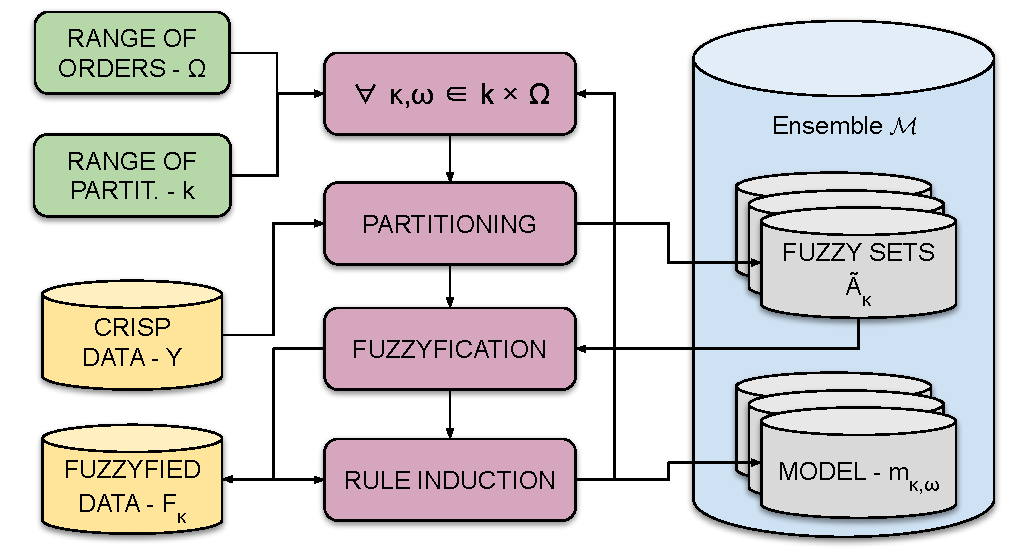
\includegraphics[width=\textwidth,height=8cm]{figures/ensemblefts_training.pdf}
\end{frame}

\note[itemize]{
\item This diagram shows the traning of the EnsembleFTS
\item The main parameters are the range of Orders and partitions
\item For each combination of orders and partitions an FTS model will be trained and stored in the ensemble
}

%%%%%%%%%%%%%%%%%%%%%%%%%%%%%%%%%%%%%%%%%%%%%%

\begin{frame}{Ensemble FTS - Forecasting Procedure}
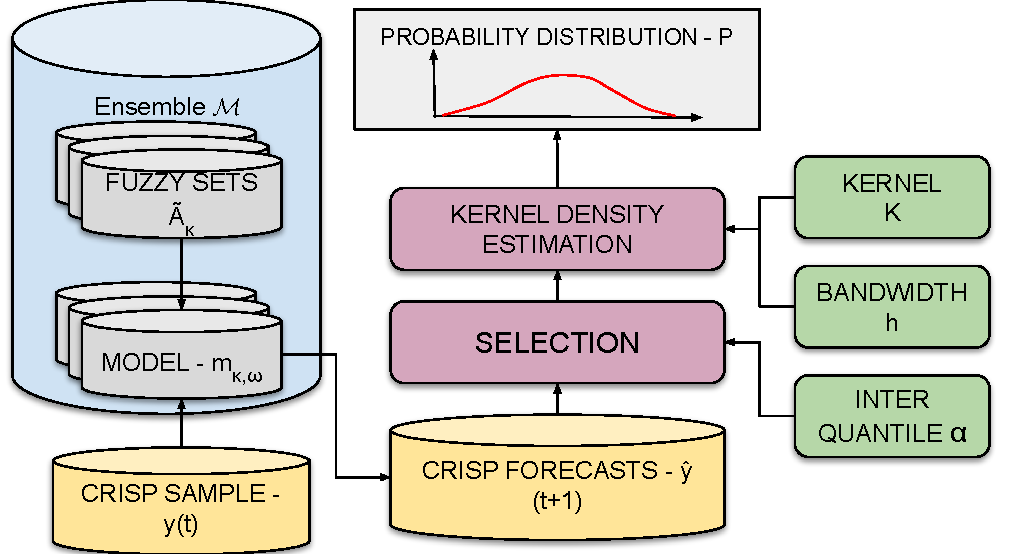
\includegraphics[width=\textwidth,height=8cm]{figures/ensemblefts_forecasting.pdf}
\end{frame}

\note[itemize]{
\item This diagram shows the forecasting process
\item The input sample is passed to each ensemble model generating the set of crisp forecasts
\item The selection remove extreme values, considering just an alpha interquantile interval
\item Then the values are smoothed in a probability distribution using a KDE
}

%%%%%%%%%%%%%%%%%%%%%%%%%%%%%%%%%%%%%%%%%%%%%%

\begin{frame}{Ensemble FTS - Sample}
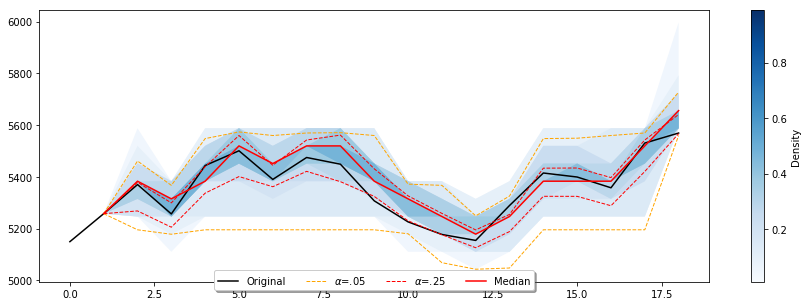
\includegraphics[width=\textwidth,height=8cm]{figures/ensemblefts_sample_onestep.png}
\end{frame}

\note[itemize]{
\item This is a sample for one step ahead probabilistic forecasting
\item The intervals are generated from the PDF using alpha levels
}

%%%%%%%%%%%%%%%%%%%%%%%%%%%%%%%%%%%%%%%%%%%%%%
\begin{frame}{Ensemble FTS - Sample}
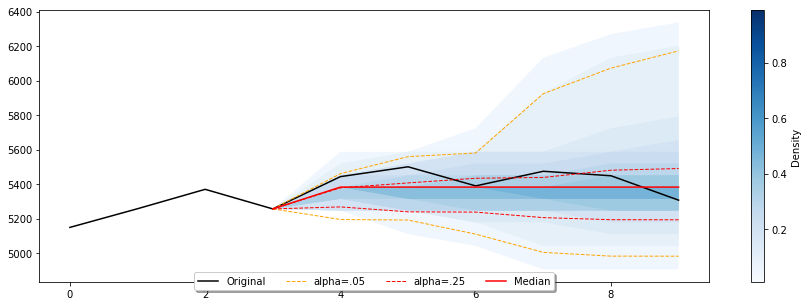
\includegraphics[width=\textwidth,height=8cm]{figures/ensemblefts_sample_manystep.png}
\end{frame}

\note[itemize]{
\item This is a sample for many steps ahead probabilistic forecasting
}

%%%%%%%%%%%%%%%%%%%%%%%%%%%%%%%%%%%%%%%%%%%%%%
\begin{frame}{Limitations of the proposed methods}
\linespread{2}
\begin{table}[]
\begin{tabular}{|c|p{4.5cm}|p{4.5cm}|} \hline
     & \begin{center}
         $\ifts$
     \end{center}& \begin{center}
         EnsembleFTS
     \end{center} \\ \hline
Pros &  \begin{tabular}{p{4cm}}
             $\bullet$ Fuzzy Uncertainty \\
             $\bullet$ Flexibility
        \end{tabular}    
        &
        \begin{tabular}{p{4cm}}
             $\bullet$ Interval Forecasting \\
             $\bullet$ Probabilistic Forecasting
        \end{tabular}
        \\ \hline
Cons &  \begin{tabular}{p{4cm}}
             $\bullet$ No confidence level \\
             $\bullet$ No probabilistic forecasting
        \end{tabular}    
        &
        \begin{tabular}{p{4cm}}
             $\bullet$ High computational cost \\
             $\bullet$ Not parsimonious
        \end{tabular} \\ \hline
\end{tabular}
\end{table}

\end{frame}

\note[itemize]{
\item The computational experiments showed that IFTS and EnsembleFTS has the same forecasting skills than the standard Mean/Variance, QAR and BSTS methods
}

%%%%%%%%%%%%%%%%%%%%%%%%%%%%%%%%%%%%%%%%%%%%%%
%%%%%%%%%%%%%%%%%%%%%%%%%%%%%%%%%%%%%%%%%%%%%%
\section{Probabilistic Weighted Fuzzy Time Series - PWFTS}

%%%%%%%%%%%%%%%%%%%%%%%%%%%%%%%%%%%%%%%%%%%%%%
\begin{frame}{Probabilistic Weighted Fuzzy Time Series - PWFTS}
\linespread{2}
\begin{itemize} 
    \item Integrated method for point, interval and probabilistic forecasting
    \item New rule based model - Fuzzy Temporal Pattern Group 
    \item Represent both the extrinsic uncertainty (fuzzy sets) and ontologic uncertainty (empirical probabilities)
\end{itemize}
\end{frame}

\note[itemize]{
\item PWFTS is the main achievement of this research and I will give more attention on it
\item Aims to be the all-in-one method
}

%%%%%%%%%%%%%%%%%%%%%%%%%%%%%%%%%%%%%%%%%%%%%%
\begin{frame}{Fuzzy Empirical Probabilities}
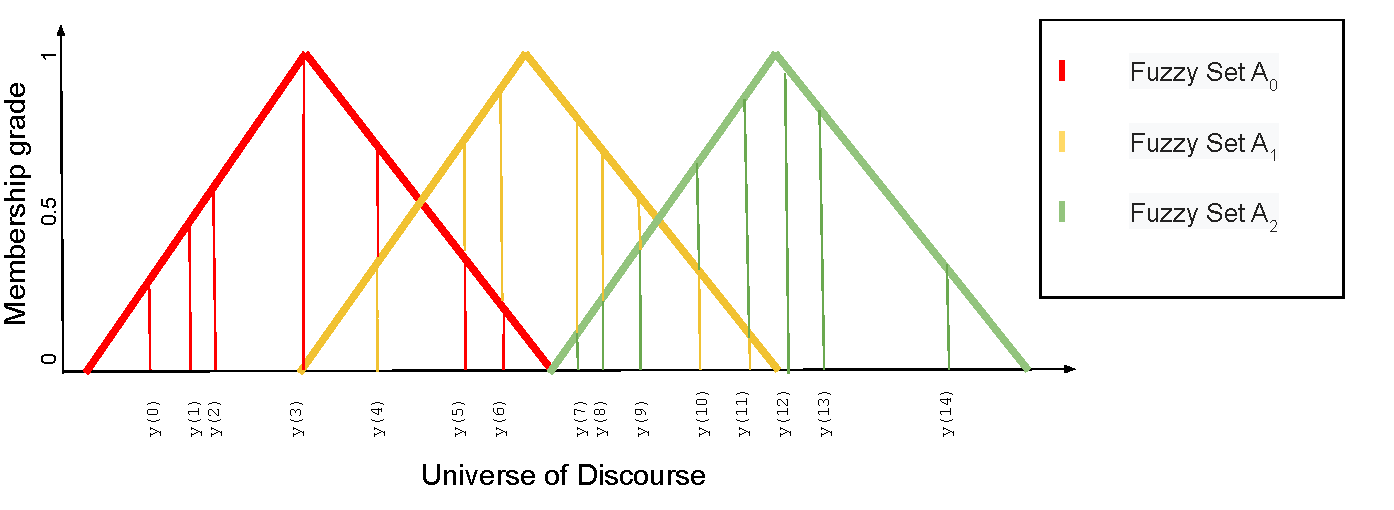
\includegraphics[width=\textwidth]{figures/pwfts_fuzzyfrequency.pdf}
$$
\begin{array}{ccc}
P(\ufset) = \frac{\sum_{y \in U} \mu_{\ufset}(y)}{\sum_{\ufset \in \ulvar}Z_{\ufset}}      & &  Z_{\ufset} = \sum_{y \in U} \mu_{\ufset}(y)
\end{array}
$$
\end{frame}


\note[itemize]{
\item Traditional probabilities are measured over crisp events, using integer counting
\item Fuzzy events do not have integer counts, but partial counts - its membership grades
\item Fuzzy frequencies are the membership degrees of the crisp values
\item the probability of a fuzzy set is the normalized sum of its fuzzy occurrences - or the sum of its memberships
\item $Z_{\ufset}$ is called Partition Function
\item the idea is to generalize the probability of the fuzzy set using the available sample
\item spread the measured occurrences over the shape and area of the membership function
}

%%%%%%%%%%%%%%%%%%%%%%%%%%%%%%%%%%%%%%%%%%%%%%
\begin{frame}{Fuzzy Empirical Probabilities}
\begin{itemize}
    \item Probability of a crisp value $y \in U$ given a fuzzy set $\ufset \in \ulvar$:
$$
P(y | \ufset) = P(\ufset) \cdot \frac{\mu_{\ufset}(y)}{Z_{\ufset}}
$$

    \item Total probability of a crisp value $y \in U$:
    
$$
P(y,\ulvar) = \sum_{\ufset \in \ulvar} P(y | \ufset)\cdot P(\ufset)
$$

\end{itemize}
\end{frame}


\note[itemize]{
\item If the empirical probability of a fuzzy set is measured by the membership of crisp events, the opposite is also possible
}

%%%%%%%%%%%%%%%%%%%%%%%%%%%%%%%%%%%%%%%%%%%%%%
\begin{frame}{PWFTS Rule Model}
\linespread{2}
$$
\begin{array}{rcl}
\pi_1 \cdot A_1 & \rightarrow &  w_{11} \cdot A_1, ..., w_{1k} \cdot A_k \\
\ldots & \ldots & \ldots \\
\pi_k \cdot A_k & \rightarrow &  w_{k1} \cdot A_1, ..., w_{kk} \cdot A_k
\end{array}
$$
\begin{itemize}
    \item $\pi_j$: \textit{Unconditional} empirical probabilities, or the probability $P(LHS)$, $\qquad\sum \pi_j = 1$
    \item $w_{ji}$: \textit{Conditional} empirical probabilities, or the probability $P(RHS|LHS)$, $\qquad\sum w_{ji} = 1$
\end{itemize}
\end{frame}

\note[itemize]{
\item Fuzzy frequencies are the membership degrees of the crisp values
\item The training process just store the frequencies and calculate the empirical probabilities with them
\item 
}

%%%%%%%%%%%%%%%%%%%%%%%%%%%%%%%%%%%%%%%%%%%%%%
\begin{frame}{PWFTS Rule Sample}
    \centering
    \begin{tabular}{rcrrr}
        $0.005\cdot A0$ & $\rightarrow$ & $0.4\cdot A0$, & $0.6\cdot A1$ &   \\
        $0.05\cdot A1$ & $\rightarrow$ & $0.05\cdot A0$, & $0.6\cdot A1$, & $0.35\cdot A2$  \\
        $0.11\cdot A2$ & $\rightarrow$ & $0.1\cdot A1$&,  $0.6\cdot A2$, & $0.3\cdot A3$  \\
        $0.14\cdot A3$ & $\rightarrow$ & $0.15\cdot A2$, & $0.6\cdot A3$, & $0.25\cdot A4$  \\
        $0.15\cdot A4$ & $\rightarrow$ & $0.2\cdot A3$, & $0.55\cdot A4$, & $0.25\cdot A5$  \\
        $0.1\cdot A5$ & $\rightarrow$ & $0.2\cdot A4$, & $0.55\cdot A5$, & $0.25\cdot A6$  \\
        $0.12\cdot A6$ & $\rightarrow$ & $0.2\cdot A5$, & $0.6\cdot A6$, & $0.2\cdot A7$  \\
        $0.09\cdot A7$ & $\rightarrow$ & $0.25\cdot A6$, & $0.55\cdot A7$, & $0.2\cdot A8$  \\
        $0.06\cdot A8$ & $\rightarrow$ & $0.25\cdot A7$, & $0.6\cdot A8$, & $0.15\cdot A9$  \\
        $0.02\cdot A9$ & $\rightarrow$ & $0.6\cdot A8$, & $0.4\cdot A9$ &   \\
    \end{tabular}
\end{frame}

\note[itemize]{
\item In this figure we can see a sample of a PWFTS model, with 10 fuzzy sets
\item In the left side are the precedent fuzzy sets with their unconditional probabilities
\item In the right side are the consequent fuzzy sets with their conditional probabilities
}

%%%%%%%%%%%%%%%%%%%%%%%%%%%%%%%%%%%%%%%%%%%%%%
\begin{frame}{PWFTS Rule Sample}
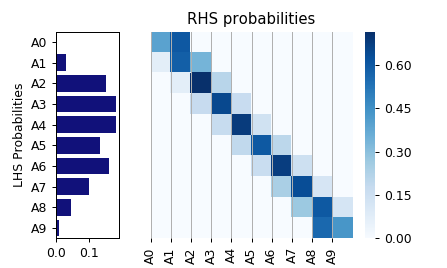
\includegraphics[width=\textwidth]{figures/pwfts_rules_firstorder.png}
\end{frame}

\note[itemize]{
\item This figure show a graphic representation of the previous PWFTS model
}

%%%%%%%%%%%%%%%%%%%%%%%%%%%%%%%%%%%%%%%%%%%%%%
\begin{frame}{Mixture Distributions}
\linespread{1.5}
How to transform the PWFTS model in a probabilistic forecast?
\begin{itemize}
    \item Each rule is a conditional probability distribution
    \item Each input crisp value "activates" one or more rules, with a different degree (its membership value)
    \item Smooth the probability distributions of each rule given:
    \begin{itemize}
        \item Membership value
        \item Unconditional proability (\textit{a priori})
    \end{itemize}
\end{itemize}
\end{frame}

\note[itemize]{
    \item
}

%%%%%%%%%%%%%%%%%%%%%%%%%%%%%%%%%%%%%%%%%%%%%%
\begin{frame}{Mixture Distributions}
How to transform the PWFTS model in a probabilistic forecast?
$$
\begin{array}{c}
     P(y) = \sum \omega_j \cdot P_j(y)  \\
     \\
     P_j: U \rightarrow [0,1] \\ 
     \\
     \sum \omega_j = 1
\end{array}
$$
\end{frame}

\note[itemize]{
    \item Smoothing distribution, is the same of mixing distributions
    \item The mixture distributions is a way to mix several distributions with the same sampling universe
    \item each probability distribution has a weight
    \item The total probability of a point is the weighted sum of its probability on each distribution
}

%%%%%%%%%%%%%%%%%%%%%%%%%%%%%%%%%%%%%%%%%%%%%%
\begin{frame}{Probabilistic Forecasting Procedure}
\linespread{2}
$$P(y(t+1)|y(t),\ulvar) = \sum_{\ufset \in \ulvar} P(y(t+1)|y(t),\ufset)\cdot P(y(t)|\ufset)\cdot P(\ufset)$$
\begin{itemize}
    \item $P(y(t+1)|y(t),\ufset)$ is related with the RHS of the rules, the conditional probability 
    \item $P(y(t)|\ufset)$ is related with the LHS of the rules, the unconditional probability
\end{itemize}
\end{frame}

\note[itemize]{
    \item Derivation of Law of Total Probability 
}

%%%%%%%%%%%%%%%%%%%%%%%%%%%%%%%%%%%%%%%%%%%%%%
\begin{frame}{PWFTS Rule Sample}
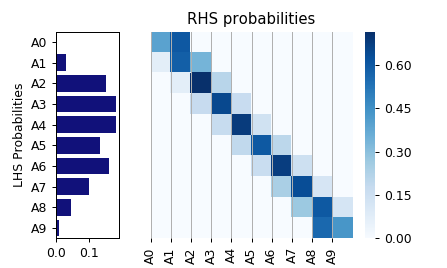
\includegraphics[width=\textwidth]{figures/pwfts_rules_firstorder.png}
\end{frame}


%%%%%%%%%%%%%%%%%%%%%%%%%%%%%%%%%%%%%%%%%%%%%%
\begin{frame}{Probabilistic Forecasting Procedure}
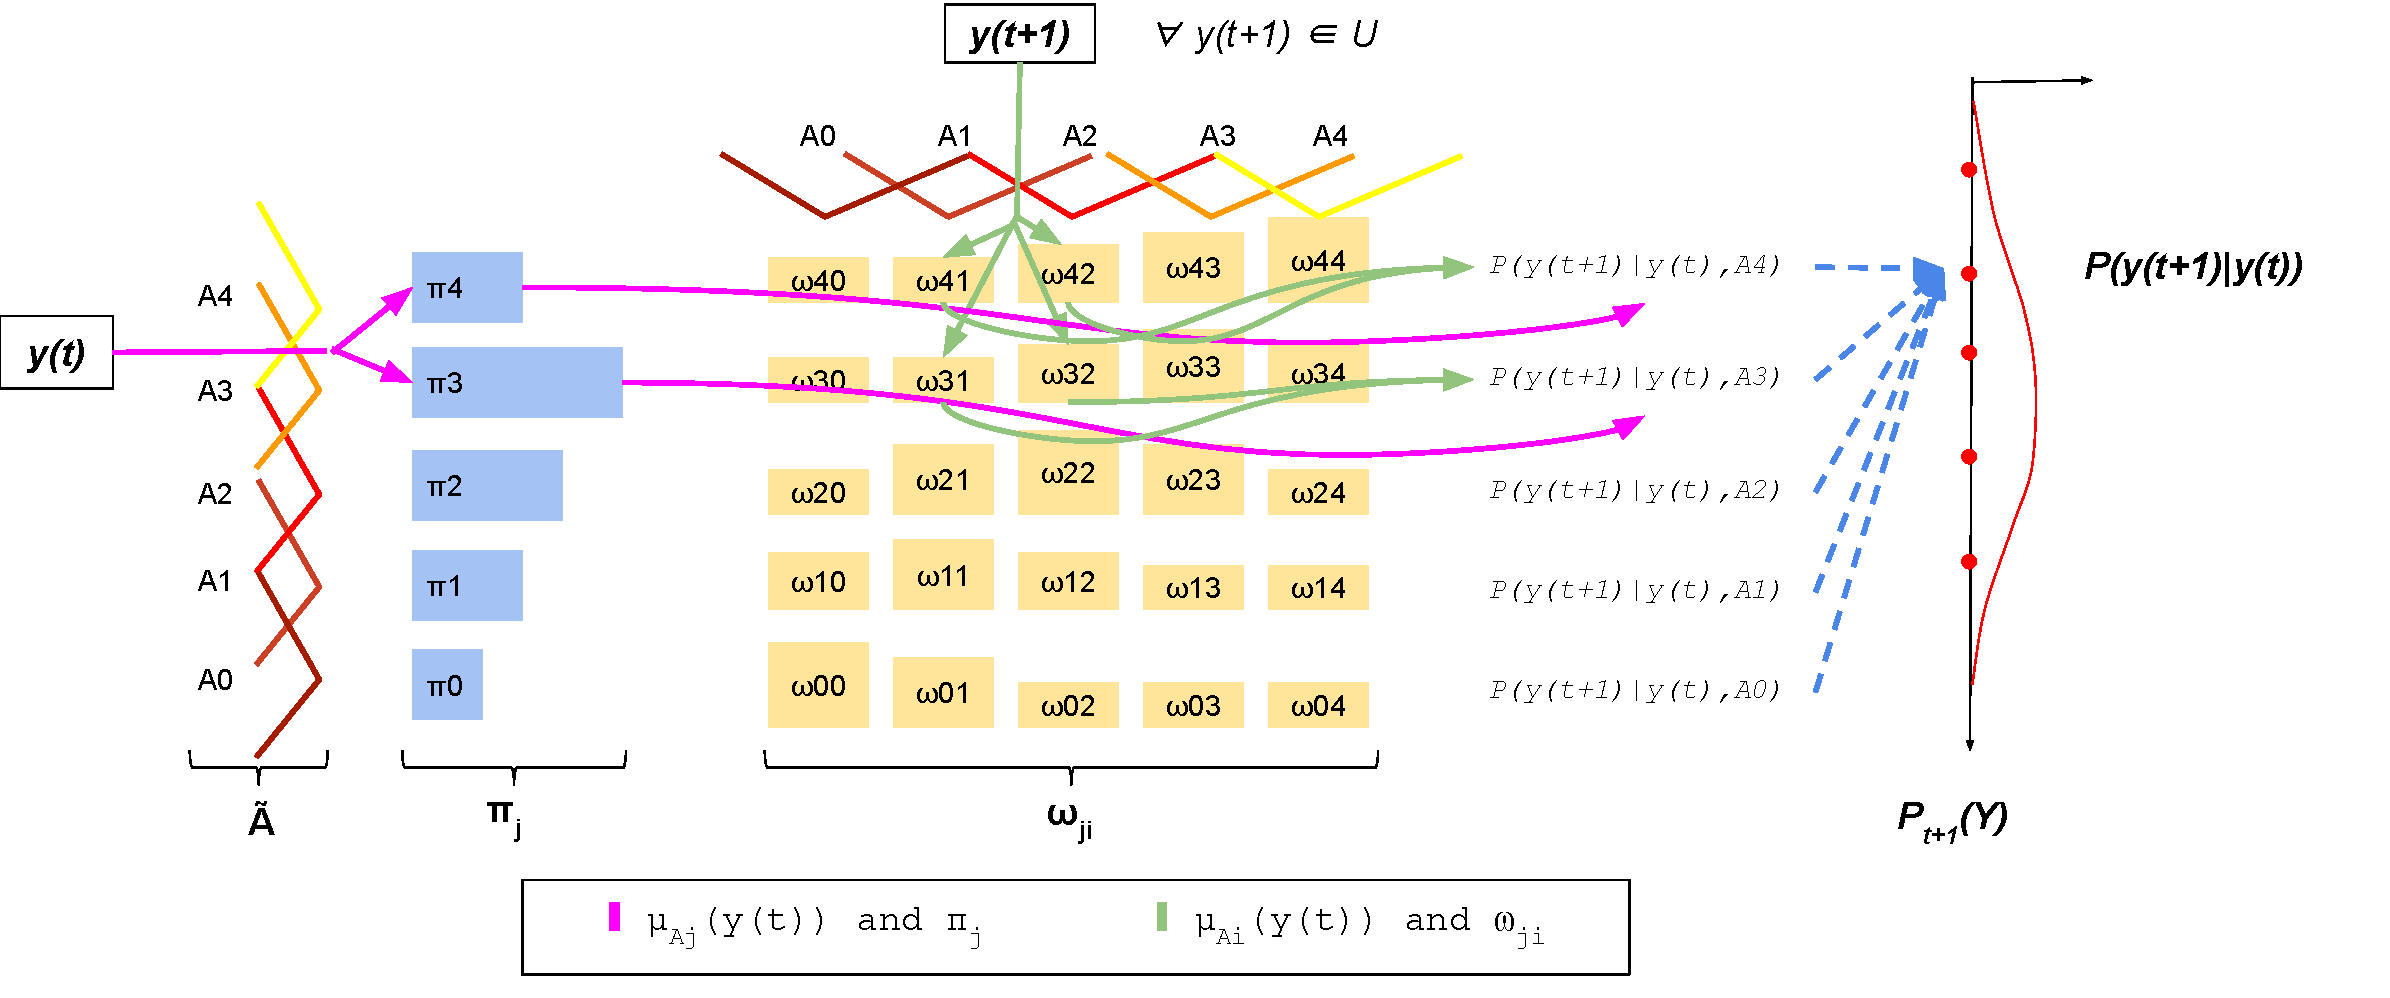
\includegraphics[width=1.1\textwidth,height=6cm]{figures/pwfts_probabilistic_forecasting.pdf}
\end{frame}


\note[itemize]{
    \item This diagram show how a probability is calculated for a point $y(t+1)$ given a input $y(t)$
}

%%%%%%%%%%%%%%%%%%%%%%%%%%%%%%%%%%%%%%%%%%%%%%
\begin{frame}{Probabilistic Forecasting Procedure}
\begin{equation}
\begin{array}{cl}
P(y(t+1) | y(t)) &=  \displaystyle \sum_{\ufset \in  \ulvar}\frac{\displaystyle P(y(t)| \ufset) \left( \sum_{i = 1}^k  P(y(t+1) | A_i,\ufset) \right)}{\displaystyle \sum_{i = 1}^k P(y(t)| A_i)}  \\
& \\
 &= \displaystyle \sum_{\ufset \in  \ulvar} \frac{ \displaystyle  \pi_j\frac{\mu_{\ufset}(y(t))}{Z_{\ufset}} \left( \sum_{i = 1}^k  w_{ji}\frac{\mu_{A_i}(y(t+1))}{Z_{A_i}} \right)}{\displaystyle \sum_{i = 1}^k \pi_i\frac{\mu_{A_i}(y(t))}{Z_{A_i}}}
\end{array}
\label{eqn:pwfts_probabilistic}
\end{equation}
\end{frame}

\note[itemize]{
    \item This is the complete equation for calculating a probability of a point $y(t+1)$ given a input $y(t)$
    \item This formula must be applied for each $y(t+1) \in U$
}

%%%%%%%%%%%%%%%%%%%%%%%%%%%%%%%%%%%%%%%%%%%%%%
\begin{frame}{PWFTS Forecasting Sample}
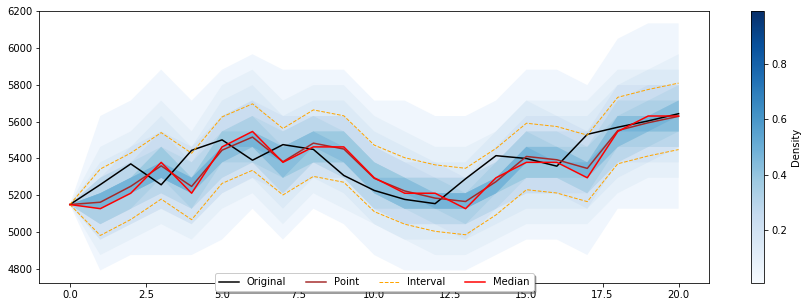
\includegraphics[width=\textwidth,height=6cm]{figures/pwfts_sample_onestep.png}
\end{frame}

\note[itemize]{
    \item This is a sample of the one step ahead performance of PWFTS
}

%%%%%%%%%%%%%%%%%%%%%%%%%%%%%%%%%%%%%%%%%%%%%%
\begin{frame}{PWFTS Forecasting Sample}
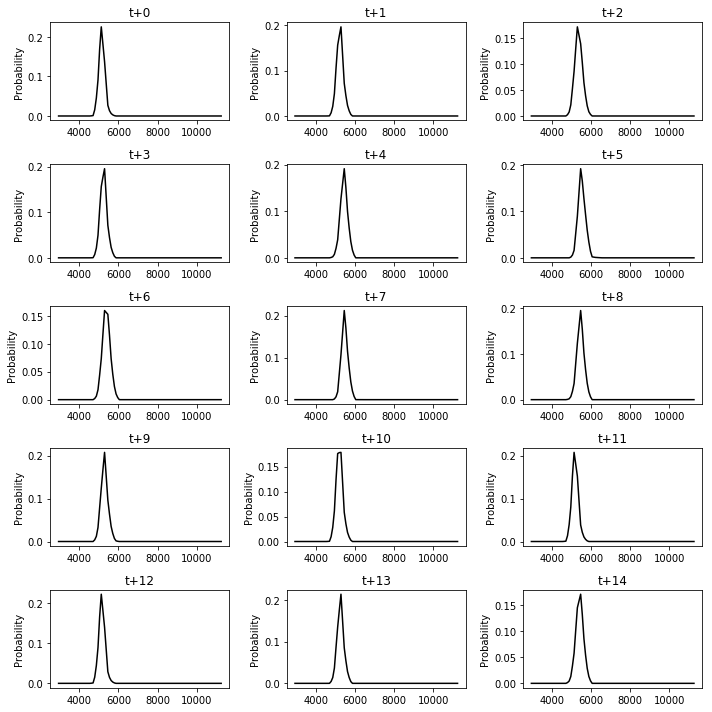
\includegraphics[width=\textwidth]{figures/pwfts_sample_onestep_tiled.png}
\end{frame}

%%%%%%%%%%%%%%%%%%%%%%%%%%%%%%%%%%%%%%%%%%%%%%
\begin{frame}{PWFTS Rule Sample}
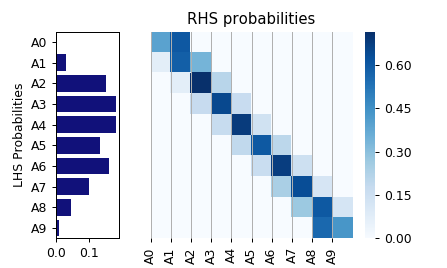
\includegraphics[width=\textwidth]{figures/pwfts_rules_firstorder.png}
\end{frame}

%%%%%%%%%%%%%%%%%%%%%%%%%%%%%%%%%%%%%%%%%%%%%%
\begin{frame}{Interval Forecasting Procedure}
$$
\begin{array}{rcl}
\intvl_j & = & \displaystyle [\underline{\mathbb{E}[ \ufset ]}\ ,\ \overline{\mathbb{E}[ \ufset ]}] \\
\underline{\mathbb{E}[ \ufset ]} & = & \sum_{A_i \in \ufset^{RHS}} w_{ji}\cdot \underline{A_i} \\ 
\overline{\mathbb{E}[ \ufset ]} & = & \sum_{A_i \in \ufset^{RHS}} w_{ji}\cdot \overline{A_i}
\end{array}
$$

$$
\begin{array}{rcl}
\mathbb{I}(t+1) & = & \displaystyle [\underline{\mathbb{E}[ \ulvar | y(t) ]}\ ,\ \overline{\mathbb{E}[ \ulvar | y(t) ]}] \\
& & \\
& = & \displaystyle \left[\frac{\sum_{\ufset \in \ulvar} P(y(t)|\ufset)\cdot \underline{\intvl_j}}{\sum_{\ufset \in \ulvar} P(y(t)|\ufset)},\frac{\sum_{\ufset \in \ulvar} P(y(t)|\ufset)\cdot \overline{\intvl_j}}{\sum_{\ufset \in \ulvar} P(y(t)|\ufset)}\right]
\end{array}
$$
\end{frame}

\note[itemize]{
    \item Once we have the probability distribution is easy to compute inter-quantile intervals with confidence level
    \item But is computationally expensive
    \item This equation is cheap and produce prediction intervals 
}

%%%%%%%%%%%%%%%%%%%%%%%%%%%%%%%%%%%%%%%%%%%%%%
\begin{frame}{Point Forecasting Procedure}

$$
\mathbb{E}[ \ufset ] = \displaystyle \sum_{i \in \ufset^{RHS}} w_{ji}\cdot mp_i
$$

$$
\estimate = \displaystyle \mathbb{E}[ \ulvar | y(t) ] =  \sum_{\ufset \in \ulvar} \frac{ P(y(t) | \ufset) \cdot \mathbb{E}[ \ufset ]} { \sum_{\ufset \in \ulvar} P(y(t) | \ufset)}
$$
\end{frame}

\note[itemize]{
    \item Once we have the probability distribution is easy to compute point forecasts with the expected value
    \item But is computationally expensive
    \item This equation is cheap and produce point forecasts close to the expected value
}

%%%%%%%%%%%%%%%%%%%%%%%%%%%%%%%%%%%%%%%%%%%%%%
%%%%%%%%%%%%%%%%%%%%%%%%%%%%%%%%%%%%%%%%%%%%%%
\section{PWFTS Extensions}


%%%%%%%%%%%%%%%%%%%%%%%%%%%%%%%%%%%%%%%%%%%%%%
\begin{frame}{High order models}
\begin{itemize}
    \item Membership of rule's precedent
$$
\displaystyle  \mu_{LHS}(y(t-L(\Omega)),\ldots,y(t-L(0)) = \bigcap_{i = \Omega}^0 \mu_{\ufset}(y(t-L(i)))
$$
    \item Conditional probability
$$
P(y(t-L(\Omega))\ldots y(t-L(0) | LHS) = \pi_{LHS} \frac{\mu_{LHS}(y(t-L(\Omega))\ldots,y(t-L(0))}{\sum_{\ufset \in LHS} Z_{\ufset}}
$$
\end{itemize}
\end{frame}

\note[itemize]{
    \item The total membership degree is the S-norm of each lag membership degree 
}

%%%%%%%%%%%%%%%%%%%%%%%%%%%%%%%%%%%%%%%%%%%%%%
\begin{frame}{High order models}
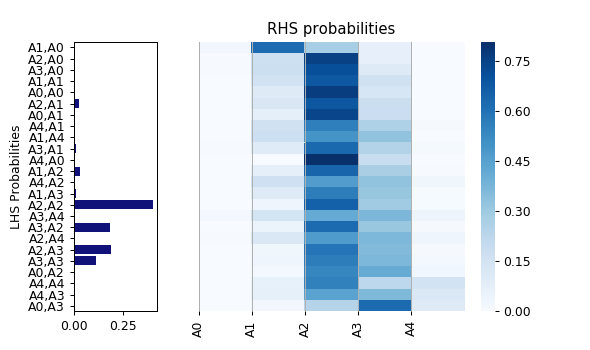
\includegraphics[width=\textwidth]{figures/pwfts_densities_secondorder.png}
\end{frame}

\note[itemize]{
    \item The figure shows a sample model of second order with just 5 fuzzy sets
    \item the models grows quickly as the order increases
}

%%%%%%%%%%%%%%%%%%%%%%%%%%%%%%%%%%%%%%%%%%%%%%
\begin{frame}{Many Steps Ahead Forecasting}
$$
\begin{array}{rcl}
P(y(h+1) | y(h))     & = &  \displaystyle \sum_{\ufset \in \ulvar} \frac{ P(y(h)| y(h-1), \ufset)}{ \sum_{i = 1}^k P(y(h)| y(h-1), A_i)}  \\
     & & \displaystyle \times  \left(  \sum_{z = 1}^k  P(y(h+1) | A_z,\ufset) \right) 
\end{array}
$$
\end{frame}

\note[itemize]{
    \item 
}

%%%%%%%%%%%%%%%%%%%%%%%%%%%%%%%%%%%%%%%%%%%%%%
\begin{frame}{Many Steps Ahead Forecasting}
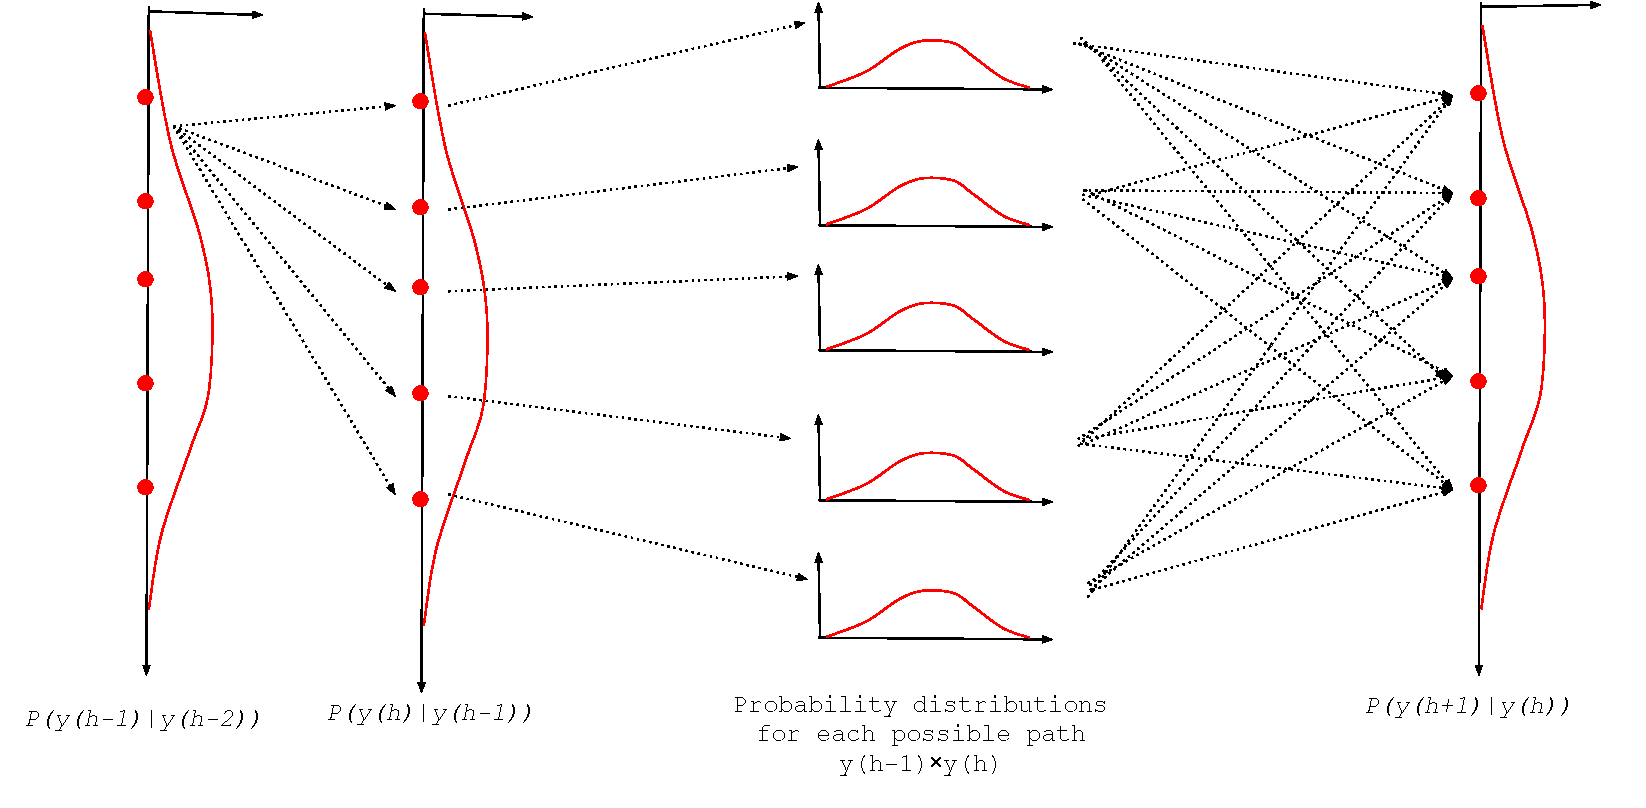
\includegraphics[width=\textwidth,height=6cm]{figures/pwfts_probabilistic_manysteps.pdf}
\end{frame}

\note[itemize]{
    \item Forecasting ahead is to forecasts probability distributions from probability distributions
    \item Computationally expensive
}

%%%%%%%%%%%%%%%%%%%%%%%%%%%%%%%%%%%%%%%%%%%%%%
\begin{frame}{Many Steps Ahead Forecasting}
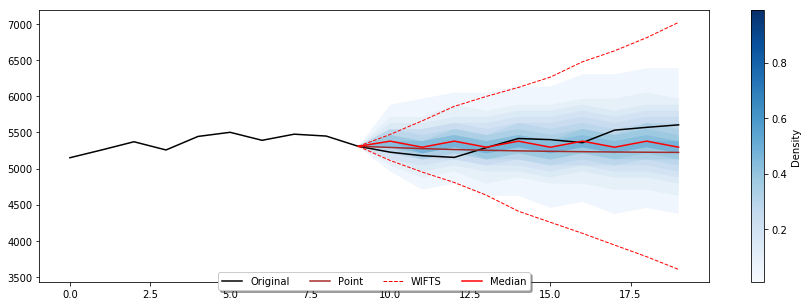
\includegraphics[width=\textwidth]{figures/pwfts_sample_manystep.png}
\end{frame}

%%%%%%%%%%%%%%%%%%%%%%%%%%%%%%%%%%%%%%%%%%%%%%
\begin{frame}{Many Steps Ahead Forecasting}
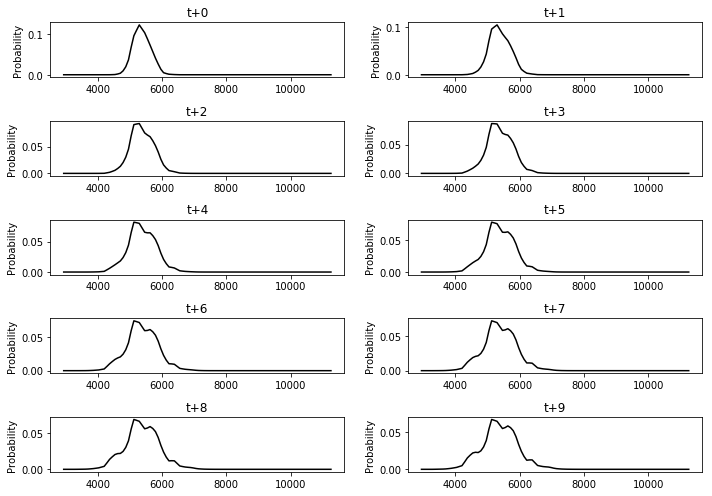
\includegraphics[width=\textwidth]{figures/pwfts_sample_manystep_tiled.png}
\end{frame}

%%%%%%%%%%%%%%%%%%%%%%%%%%%%%%%%%%%%%%%%%%%%%%
%%%%%%%%%%%%%%%%%%%%%%%%%%%%%%%%%%%%%%%%%%%%%%
\section{PWFTS Computational Experiments}

%%%%%%%%%%%%%%%%%%%%%%%%%%%%%%%%%%%%%%%%%%%%%%
\begin{frame}{Point Forecasting}
\begin{table}[htb]
\resizebox{\textwidth}{!}{% <------ Don't forget this %
\centering
    \begin{tabular}{|c|ccccccc|}
\hline
\textbf{Dataset} & \textbf{ARIMA} & \textbf{QAR} & \textbf{PWFTS} & \textbf{WHOFTS} & \textbf{HOFTS} & \textbf{kNN} & \textbf{BSTS} \\
\hline
\multirow{2}{*}{S\&P 500} &     6.091 &     8.177 &    10.541 &    12.822 &    13.605 &    19.242 &    380.466 \\
 &   $\pm$7.452 &  $\pm$11.366 &   $\pm$10.19 &  $\pm$11.336 &  $\pm$12.392 &   $\pm$24.97 &  $\pm$947.809 \\ \hline
\multirow{2}{*}{NASDAQ} &    22.592 &    17.951 &    24.839 &    27.154 &    29.713 &    34.742 &    413.494 \\
 &  $\pm$24.991 &  $\pm$11.965 &  $\pm$18.198 &   $\pm$15.05 &  $\pm$12.875 &  $\pm$25.096 &  $\pm$837.281 \\ \hline
\multirow{2}{*}{TAIEX} &    91.311 &      66.9 &    75.558 &    90.433 &   100.787 &    80.213 &     271.66 \\
 &  $\pm$63.249 &  $\pm$44.369 &  $\pm$56.739 &   $\pm$58.93 &  $\pm$62.932 &  $\pm$56.494 &  $\pm$250.078 \\ \hline
\end{tabular}
}
    \caption{RMSE for one step ahead point forecasts}
    \label{tab:pwfts_point_results}
\end{table}

\begin{table}[hbt]
\small
    \centering
    \begin{tabular}{|c|c|}
\hline
       METHOD &       RANK \\
\hline
QAR &   6.333333 \\
ARIMA &   7.333333 \\
PWFTS &   8.333333 \\
WHOFTS &  10.333333 \\
HOFTS &  12.000000 \\
kNN &  12.666667 \\
BSTS &  20.000000 \\
\hline
\end{tabular}
    \caption{Friedman aligned ranks for point forecasts}
    \label{tab:pwfts_point_ranks}
\end{table}
\end{frame}

\note[itemize]{
    \item The point forecasting experiments showed that PWFTS improves HOFTS and WHOFTS
    \item PWFTS performs as good as ARIMA and QAR
}

%%%%%%%%%%%%%%%%%%%%%%%%%%%%%%%%%%%%%%%%%%%%%%
\begin{frame}{Interval Forecasting}
\begin{table}[htb]
\resizebox{\textwidth}{!}{% <------ Don't forget this %
\centering
\begin{tabular}{|c|cccccccc|}
\hline
\textbf{Dataset} & \textbf{ARIMA} & \textbf{PWFTS} & \textbf{QAR} & \textbf{WIFTS} & \textbf{IFTS} & \textbf{kNN} & \textbf{EnsembleFTS} & \textbf{BSTS} \\ \hline
\multirow{2}{*}{S\&P 500} &      72.712 &    73.505 &    121.694 &    111.705 &    113.516 &    131.394 &     268.567 &     292.415 \\
 &   $\pm$135.871 &   $\pm$99.09 &  $\pm$319.305 &  $\pm$156.013 &   $\pm$91.627 &   $\pm$166.31 &   $\pm$318.259 &   $\pm$384.499 \\ \hline
\multirow{2}{*}{NASDAQ} &     233.261 &   112.944 &    106.416 &     123.35 &    284.692 &    170.709 &     603.881 &     652.036 \\
 &   $\pm$486.735 &  $\pm$33.666 &   $\pm$56.248 &  $\pm$141.251 &   $\pm$147.24 &  $\pm$156.097 &   $\pm$638.297 &   $\pm$963.624 \\ \hline
\multirow{2}{*}{TAIEX} &     858.124 &   348.647 &        340 &    480.581 &    917.879 &    428.484 &     898.531 &     1280.67 \\
 &  $\pm$1337.139 &  $\pm$82.036 &   $\pm$269.34 &  $\pm$561.826 &  $\pm$243.737 &  $\pm$269.459 &  $\pm$1175.107 &  $\pm$1472.031 \\ \hline
\end{tabular}
}
    \caption{Average Winkler Score with $\alpha=.05$ for one step ahead interval forecasts}
    \label{tab:pwfts_interval_results}
\end{table}

\begin{table}[hbt]
\small
    \centering
    \begin{tabular}{|c|c|}
\hline
       METHOD &       RANK \\
\hline
PWFTS &   6.000000 \\
QAR &   6.666667 \\
WIFTS &   7.666667 \\
kNN &   8.666667 \\
ARIMA &  13.000000 \\
IFTS &  16.666667 \\
EnsembleFTS &  19.666667 \\
BSTS &  21.666667 \\
\hline
\end{tabular}
    \caption{Friedman aligned ranks for interval forecasts }
    \label{tab:pwfts_interval_ranks}
\end{table}
\end{frame}

%%%%%%%%%%%%%%%%%%%%%%%%%%%%%%%%%%%%%%%%%%%%%%
\begin{frame}{Interval Forecasting}
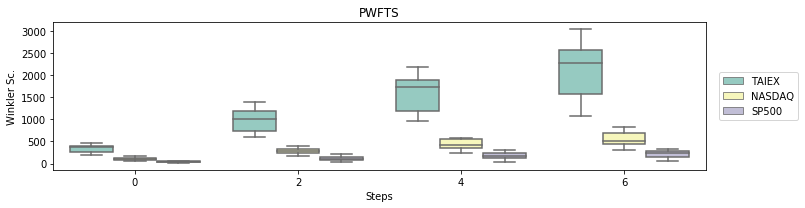
\includegraphics[width=\textwidth]{figures/pwfts_ahead_interval.png}
\end{frame}

%%%%%%%%%%%%%%%%%%%%%%%%%%%%%%%%%%%%%%%%%%%%%%
\begin{frame}{Probabilistic Forecasting}
\begin{table}[htb]
\resizebox{\textwidth}{!}{% <------ Don't forget this %
\centering
\begin{tabular}{|c|cccccc|}
\hline
\textbf{Dataset} & \textbf{PWFTS} & \textbf{QAR} & \textbf{kNN} & \textbf{ARIMA} & \textbf{EnsembleFTS} & \textbf{BSTS} \\
\hline
\multirow{2}{*}{NASDAQ} &    0.882 &    1.028 &    1.158 &    1.444 &       1.923 &    3.208 \\
 &  $\pm$0.347 &  $\pm$0.748 &  $\pm$0.477 &  $\pm$1.303 &     $\pm$1.416 &  $\pm$3.983 \\ \hline
\multirow{2}{*}{TAIEX} &    0.967 &    1.135 &    1.229 &    1.691 &       1.301 &    4.081 \\
 &  $\pm$0.404 &  $\pm$0.613 &  $\pm$0.693 &  $\pm$1.239 &     $\pm$1.118 &  $\pm$5.306 \\ \hline
\multirow{2}{*}{S\&P 500} &    1.257 &    1.557 &    4.403 &    1.216 &       1.995 &    3.278 \\
 &  $\pm$0.722 &   $\pm$1.74 &  $\pm$3.261 &  $\pm$1.166 &     $\pm$2.255 &   $\pm$3.16 \\ \hline
\end{tabular}
}
    \caption{CRPS for one step ahead interval forecasts}
    \label{tab:pwfts_probabilistic_results}
\end{table}

\begin{table}[hbt]
\small
    \centering
    \begin{tabular}{|c|c|}
\hline
       METHOD &       RANK \\
\hline
PWFTS &   3.333333 \\
QAR &   5.666667 \\
ARIMA &   8.666667 \\
kNN &  11.333333 \\
EnsembleFTS &  11.666667 \\
BSTS &  16.333333 \\ \hline
\end{tabular}
    \caption{Friedman aligned ranks for probabilistic forecasts }
    \label{tab:pwfts_probabilistic_ranks}
\end{table}
\end{frame}

%%%%%%%%%%%%%%%%%%%%%%%%%%%%%%%%%%%%%%%%%%%%%%
\begin{frame}{Probabilistic Forecasting}
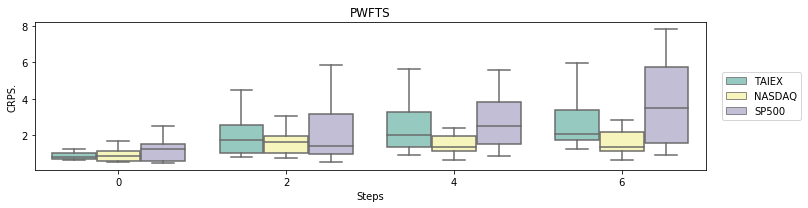
\includegraphics[width=\textwidth]{figures/pwfts_ahead_probabilistic.png}
\end{frame}

%%%%%%%%%%%%%%%%%%%%%%%%%%%%%%%%%%%%%%%%%%%%%%
\begin{frame}{PWFTS}
\linespread{2}
\begin{itemize}
    \item Versatility
    \begin{itemize}
        \item Point, interval and probabilistic forecasting
        \item For one to many steps ahead
    \end{itemize}
    \item Flexibility
    \item Accuracy
    \item Computational Cost
\end{itemize}
\end{frame}

%%%%%%%%%%%%%%%%%%%%%%%%%%%%%%%%%%%%%%%%%%%%%%
%%%%%%%%%%%%%%%%%%%%%%%%%%%%%%%%%%%%%%%%%%%%%%
\section{Scalability}

%%%%%%%%%%%%%%%%%%%%%%%%%%%%%%%%%%%%%%%%%%%%%%
\begin{frame}{Distributed Testing}
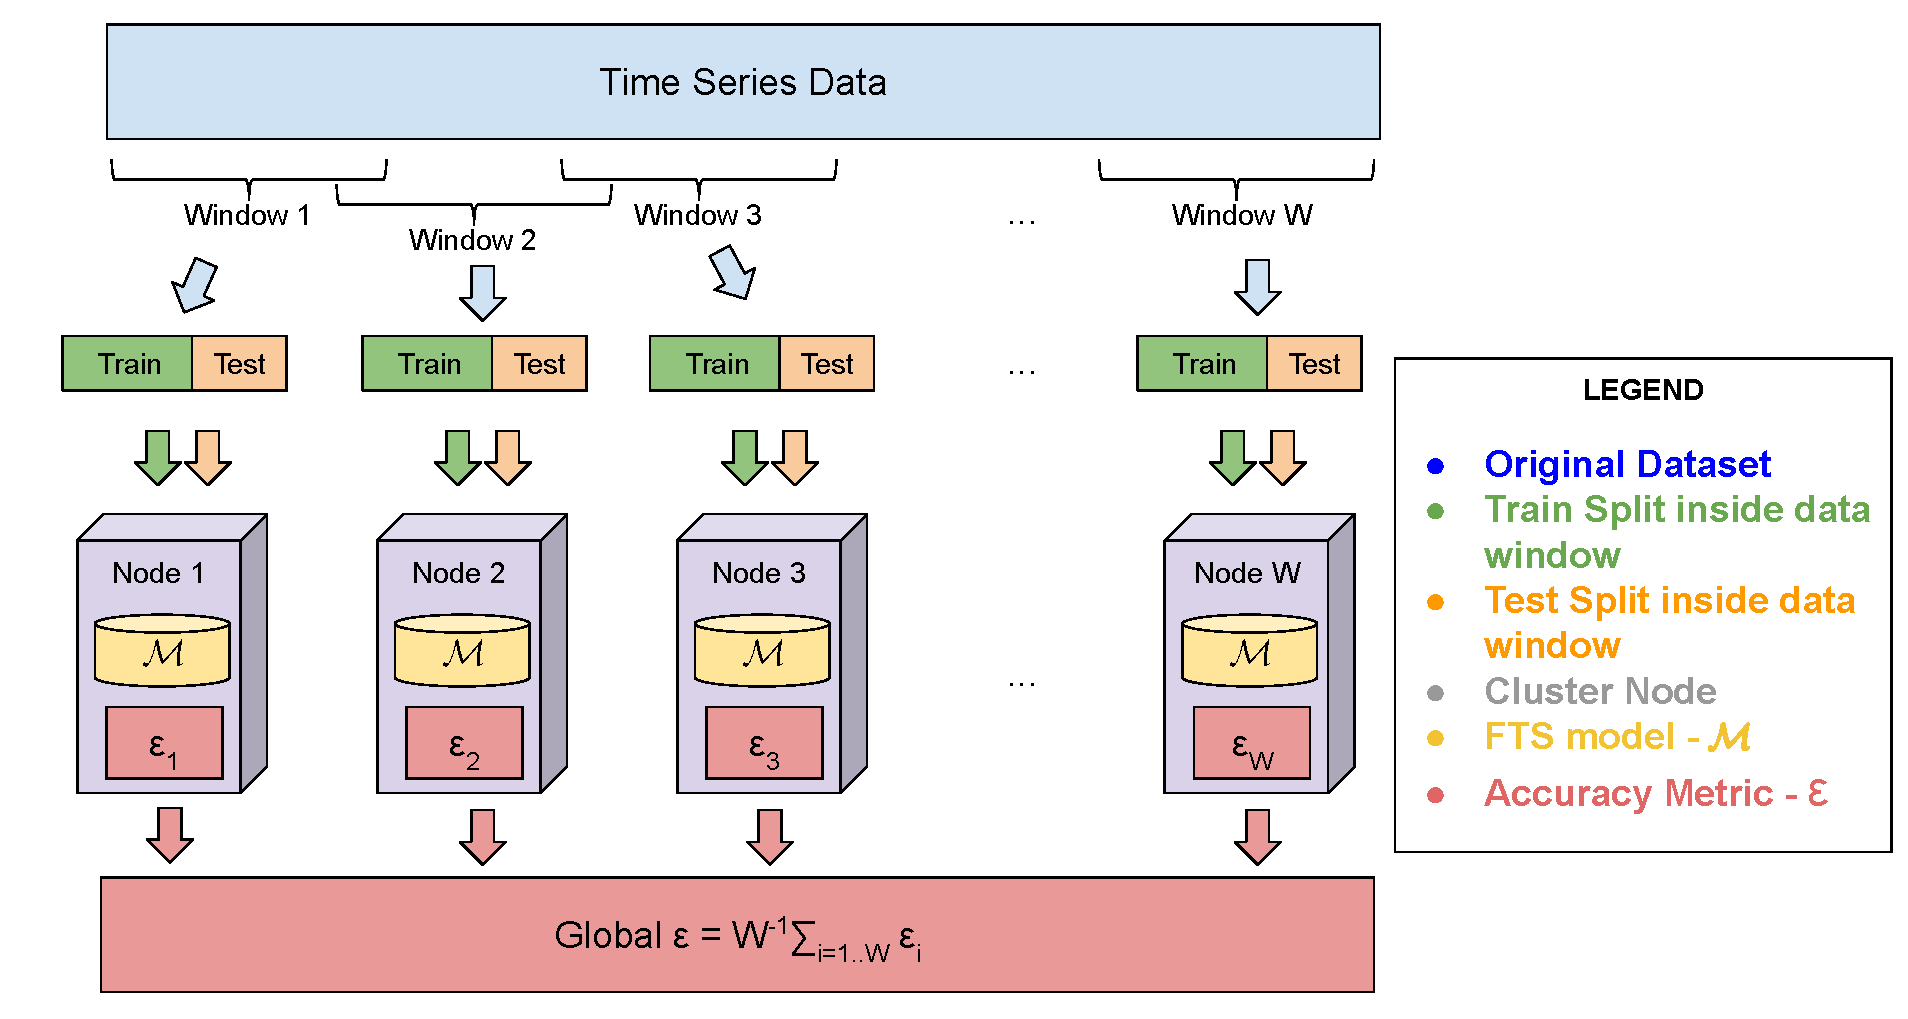
\includegraphics[width=\textwidth]{figures/distributed_testing.pdf}
\end{frame}

\note[itemize]{
    \item This figure shows the common experimentation set up for time series
    \item it is collend rolling window, or sliding window cross validation
    \item time series are divided in smaller and overlapping data sets called windows
    \item each window is divided again in train/test subsets and a model is trainined and teste with this data
    \item later the results are gathered and aggregated
}

%%%%%%%%%%%%%%%%%%%%%%%%%%%%%%%%%%%%%%%%%%%%%%
\begin{frame}{Distributed Models}
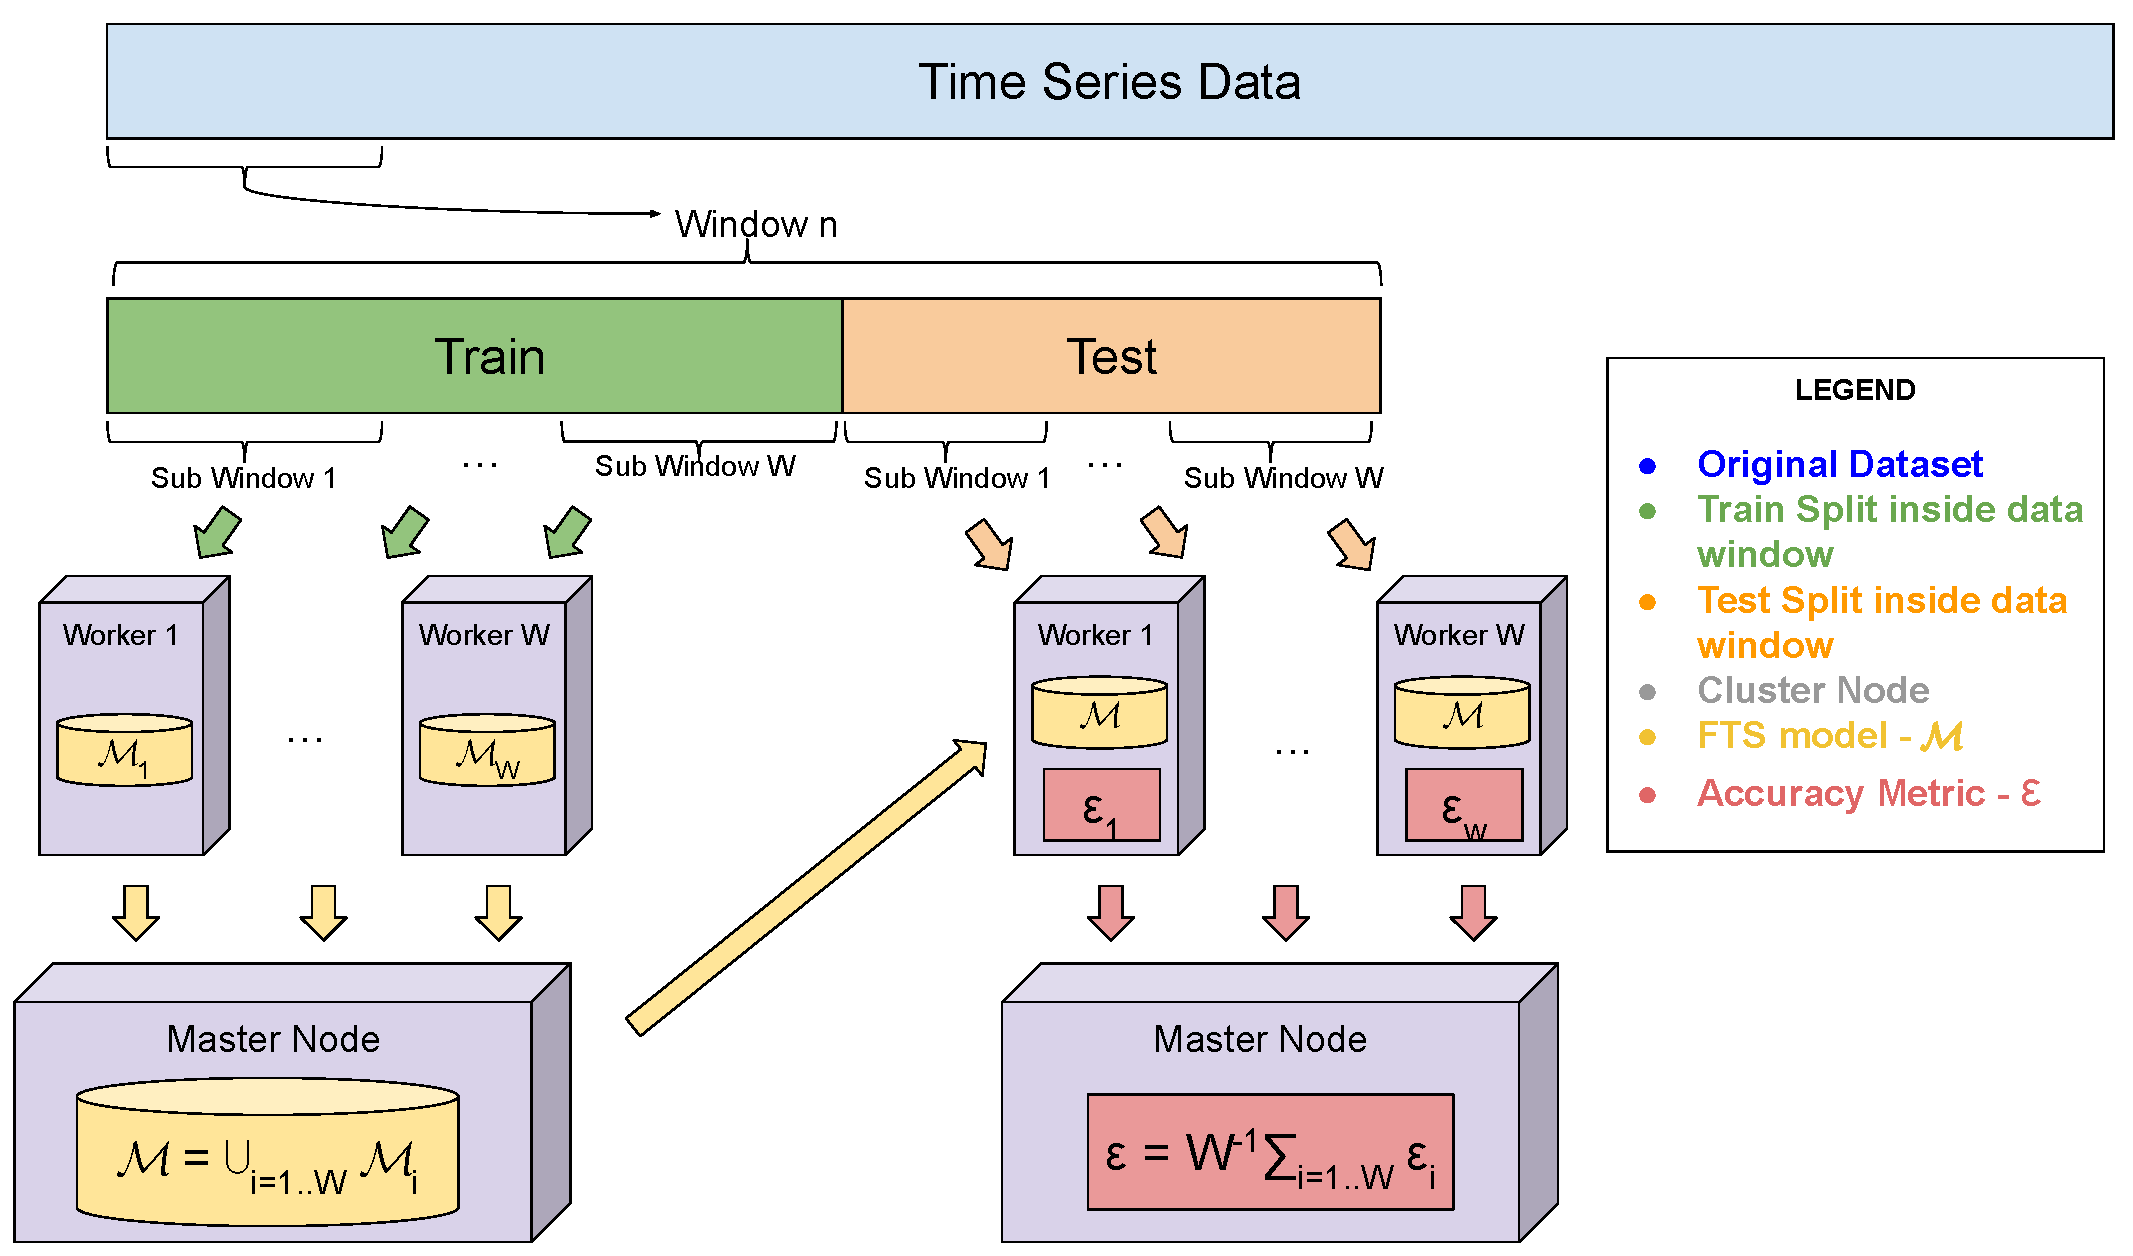
\includegraphics[width=\textwidth]{figures/distributed_models.pdf}
\end{frame}

\note[itemize]{
    \item Sometimes the time series is so big that even dat windows dot not fit in the memory of a single machine
    \item Decrease the size of the window can produce non-significant results
    \item the solution is to distribute the training procedure over several machines
    \item then merge the individual models into a single unique model
    \item this is possible because of the rule based knowledge model and its white box design
    \item this is also one of the key features of the rule-based models
}


%%%%%%%%%%%%%%%%%%%%%%%%%%%%%%%%%%%%%%%%%%%%%%
\begin{frame}{Distributed Models}
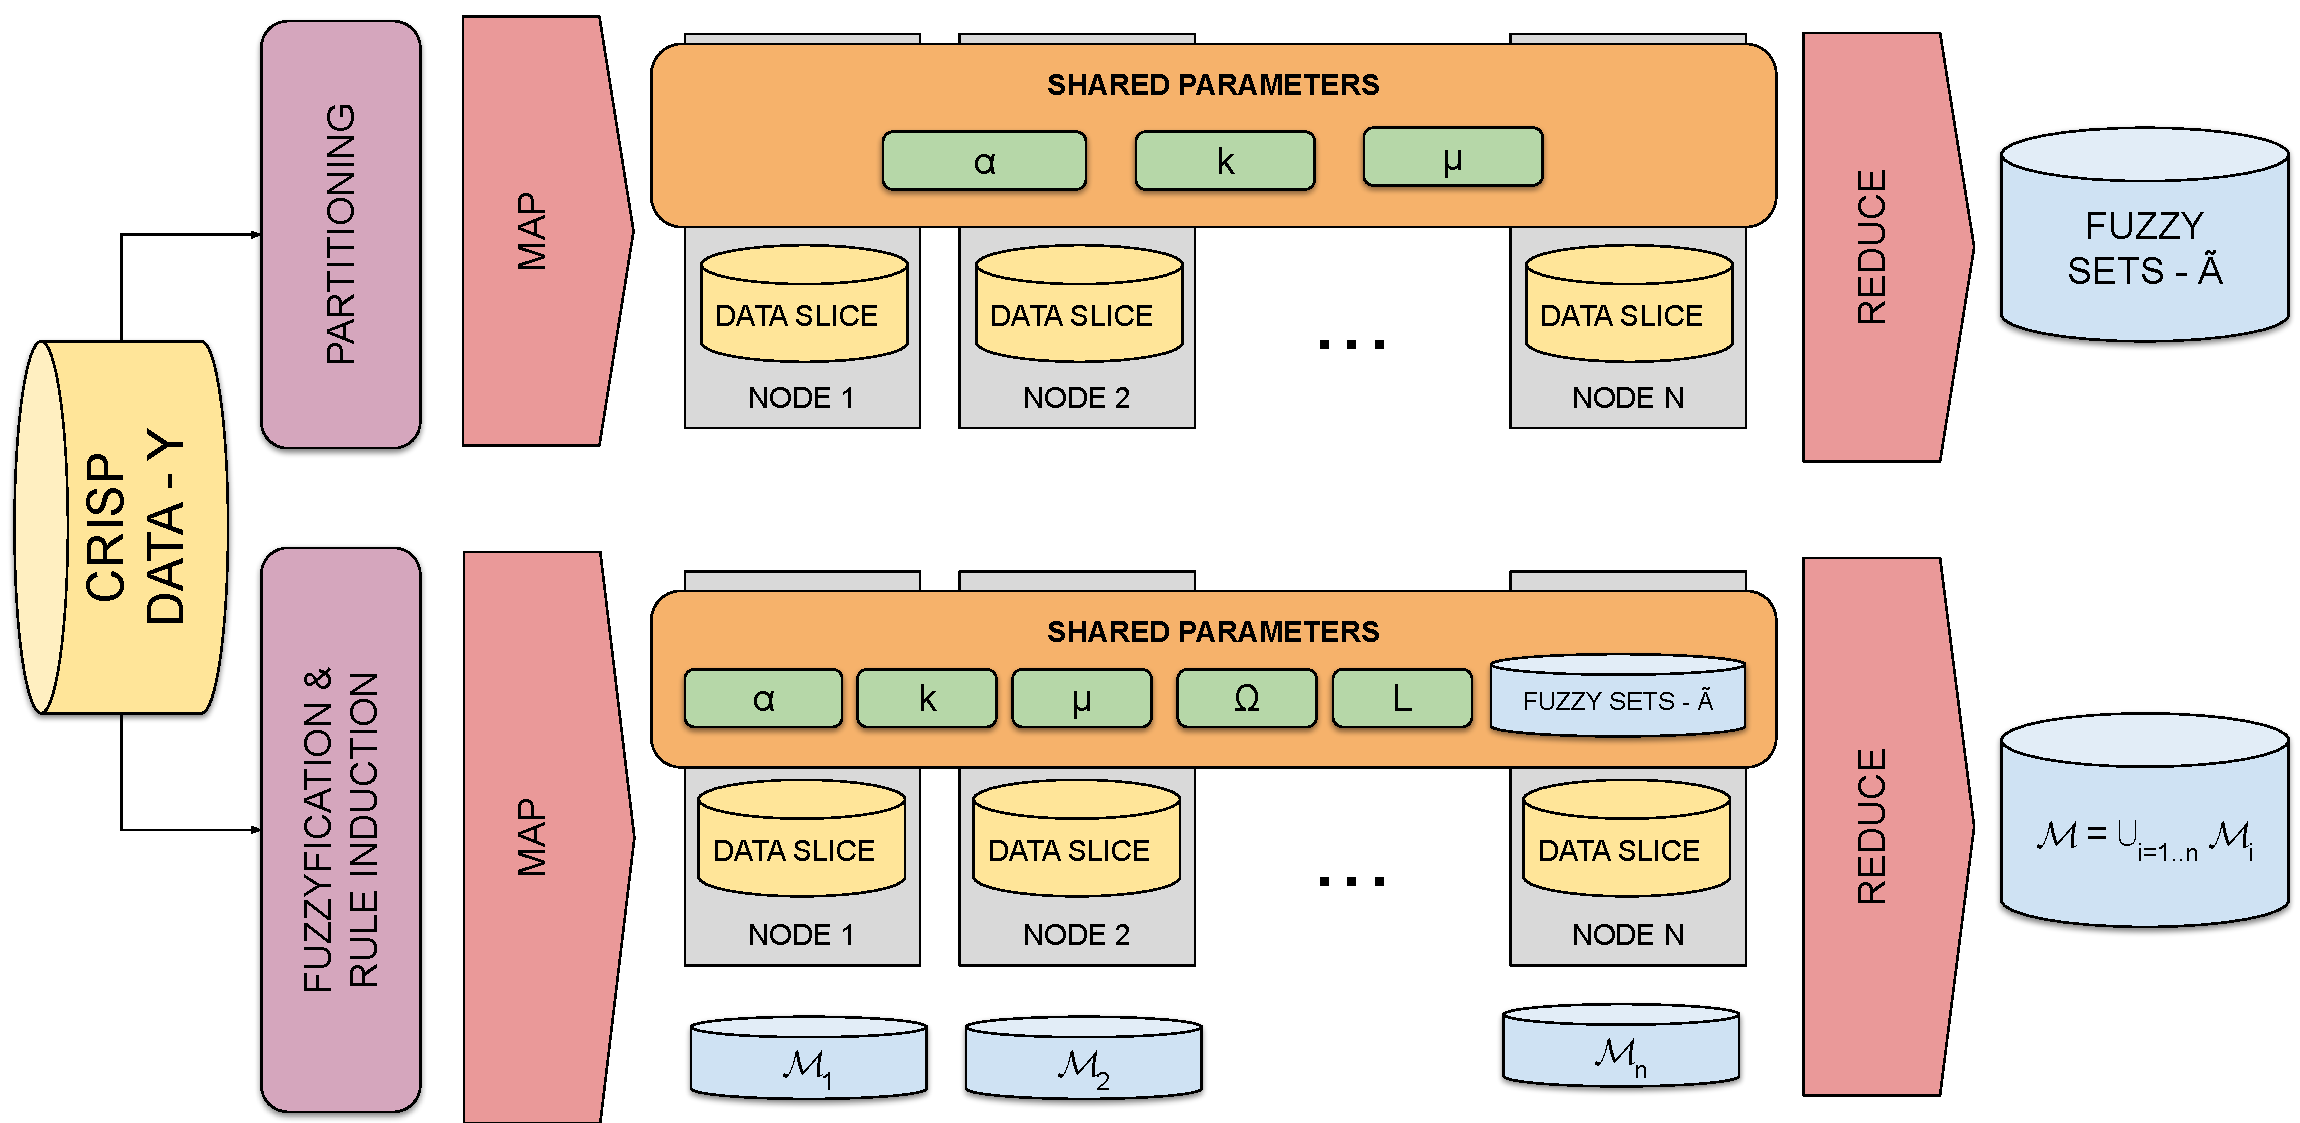
\includegraphics[width=\textwidth]{figures/distributed_models_training.pdf}
\end{frame}

\note[itemize]{
    \item This diagram show how the processes are implemented using the Map/Reduce paradigm using, for instancem, Hadoop or Spark frameworks and implemented on cheap commodity hardware
}

%%%%%%%%%%%%%%%%%%%%%%%%%%%%%%%%%%%%%%%%%%%%%%
\begin{frame}{Distributed Models - Speed Up by Number of CPU's}
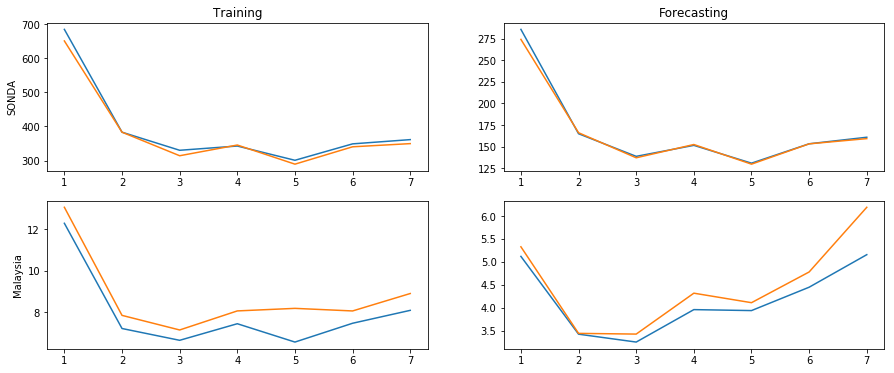
\includegraphics[width=\textwidth]{figures/speed_up.png}
\end{frame}

\note[itemize]{
    \item Using the distributed training on a not big time series is not profitable due to network overhead
    \item we should use it only on big time series
}

%%%%%%%%%%%%%%%%%%%%%%%%%%%%%%%%%%%%%%%%%%%%%%
%%%%%%%%%%%%%%%%%%%%%%%%%%%%%%%%%%%%%%%%%%%%%%
\section{Distributed Evolutionary Hyperparameter Optimization - DEHO}


%%%%%%%%%%%%%%%%%%%%%%%%%%%%%%%%%%%%%%%%%%%%%%
\begin{frame}{Hyperparameter Optimization}
\linespread{2}
$$\hat{\theta} = \arg\min_\theta f(\Theta)$$
\begin{itemize}
    \item $\theta \in \Theta$:  The set of hyperparameters 
    \item $f: \Theta \rightarrow \mathbb{R}^+$: Loss function
    \item Objective Functions
    \begin{itemize}
        \item Accuracy - $f_1$
        \item Parsimony - $f_2$
    \end{itemize}
\end{itemize}
\end{frame}

\note[itemize]{
    \item The hyperparameter optimization problem is to find the valus of each hyperparameter, given a set of hyperparameters, that minimize the loss function
    \item In our case, the loss function is composed by two metrics
    \item Accuracy is related with the error of the model
    \item Parsimony is related with the number of parameters of the model
}

%%%%%%%%%%%%%%%%%%%%%%%%%%%%%%%%%%%%%%%%%%%%%%
\begin{frame}{Distributed Evolutionary Hyperparameter Optimization}
\scriptsize
\textbf{Optimize}:
$$
\begin{array}{cc}
    minimize \quad  f_1  = & \quad 0.6\bar{\epsilon} + 0.4\sigma_\epsilon \\
    minimize \quad  f_2  = & \quad 0.6|\mathcal{M}| + 0.4|L|  
\end{array}
$$

\textbf{Where:}
$$
\begin{array}{ccc}
RMSE = \sqrt{\sum_{t=0}^n (y(t) - \hat{y}(t))^2 )} & &
\bar{\epsilon}  =  W^{-1}\sum_{i=0}^W RMSE(i) \\ 
\\
\sigma_\epsilon  =  W^{-1}\sum_{i=0}^W \bar{\epsilon} - RMSE(i) & & |\model| = \sum_{i=0}^{rules} 1 \\ 
\\
|L| = \sum_{i=0}^{\Omega-1} L(i)  & &
\end{array}
$$

\textbf{Subject to}:

$$
\begin{array}{ccc}
\Omega &\geq & 1 \\
k &\geq & 3  \\
\alpha &\in & [0,1)  \\
1 \leq & L(0) < & ... < L(\Omega)  
\end{array}
$$
\end{frame}

%%%%%%%%%%%%%%%%%%%%%%%%%%%%%%%%%%%%%%%%%%%%%%
\begin{frame}{Genetic Algorithm}
\linespread{2}
\begin{itemize}
    \item Hyperparameter: $\Theta = \{\mu,k,\alpha,\Omega,L\}$
    \item Genotype: the values of each hyperparameter $\theta \in \Theta$
    \item Fenotype/Evaluation: distributed training/testing with sliding window cross validation
    \item Selection: Double Tournament strategy 
\end{itemize}
\end{frame}

\note[itemize]{
    \item Vanilla GA are used for monovariate problems
    \item Our implementation uses the Double Tournament to balance the two objectives
}

%%%%%%%%%%%%%%%%%%%%%%%%%%%%%%%%%%%%%%%%%%%%%%
\begin{frame}{Distributed Evolutionary Hyperparameter Optimization}
\begin{table}[htb]
    \centering
    \begin{tabular}{|c|p{7cm}|} \hline
        \textbf{Parameter} & \textbf{Description}  \\ \hline
         $PS \in \mathbb{N}^+$ & Population Size \\ \hline
         $NG \in \mathbb{N}^+$ & Max Number of Generations \\ \hline 
         $0 < NG_{stop} < NG$ & Max Number of Generations without improvement \\ \hline 
         $SR \in [0,1]$ & Selection Rate \\ \hline 
         $CR \in [0,1]$ & Crossover Rate \\ \hline 
         $MR \in [0,1]$ & Mutation Rate \\ \hline 
    \end{tabular}
    \caption{Genetic Algorithm parameters}
    \label{tab:genetic_algoritm}
\end{table}
\end{frame}

%%%%%%%%%%%%%%%%%%%%%%%%%%%%%%%%%%%%%%%%%%%%%%
\begin{frame}{Distributed Evolutionary Hyperparameter Optimization}
\begin{table}[htb]
    \centering
    \begin{tabular}{|c|c|c|} \hline
        \textbf{Parameter} & \textbf{Dataset} & \textbf{Value} \\ \hline
         \multirow{4}{*}{$W_L$}  & 
         \begin{tabular}{c}
              SONDA  \\
              Wind Speed 
         \end{tabular} & 600,000 \\ \cline{2-3}
                & 
        \begin{tabular}{c}
              SONDA  \\
              Solar Radiation  
         \end{tabular} & 600,000 \\ \cline{2-3}
                & 
        \begin{tabular}{c}
              Malaysia  \\
              Temperature  
         \end{tabular} & 10,000 \\ \cline{2-3}
                & 
        \begin{tabular}{c}
              Malaysia  \\
              Eletric Load  
         \end{tabular} & 10,000 \\ \hline
         $W_I$ & All &  .5 \\ \hline
         $T_S$ &  All &.9  \\ \hline
         $PS$ &  All &20  \\ \hline
         $NG$ &  All &30  \\ \hline 
         $NG_{stop}$  &  All &10  \\ \hline 
         $SR$ &  All &.5  \\ \hline 
         $CR$ &  All &.5  \\ \hline 
         $MR$ &  All &.2  \\ \hline  
    \end{tabular}
    \caption{Distributed Evolutive Hyperparameter Optimization parameter values}
    \label{tab:hyperopt_parameters}
\end{table}
\end{frame}


%%%%%%%%%%%%%%%%%%%%%%%%%%%%%%%%%%%%%%%%%%%%%%
\begin{frame}{DEHO Convergence}
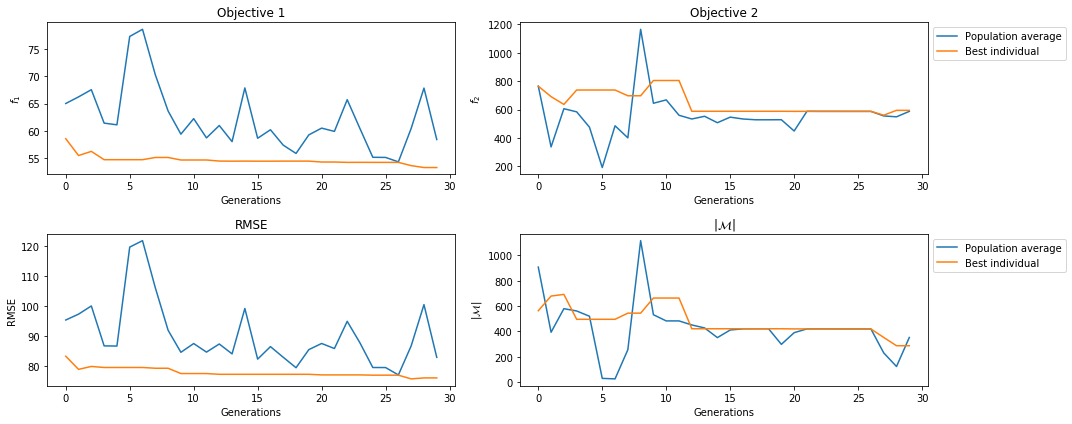
\includegraphics[width=\textwidth,height=6cm]{figures/deho_convergence.png}
\end{frame}

\note[itemize]{
    \item DEHO converges fast
    \item The design of the algorithm favor the accuracy over the parsimony but in general the both are well balanced
}

%%%%%%%%%%%%%%%%%%%%%%%%%%%%%%%%%%%%%%%%%%%%%%
\begin{frame}{DEHO}

\begin{table}[htb]
\resizebox{\textwidth}{!}{% <------ Don't forget this %
\begin{tabular}{|c|c|c|c|c|c|c|c|c|}
\hline
\textbf{Dataset}                       & \textbf{Generations}                                                            & $\mathbf{k}$                                                                   & $\mathbf{\mu}$     & $\mathbf{\alpha}$                                                              & $\mathbf{\Omega}$  & $\mathbf{L}$               & \textbf{Metric} & \textbf{Value}                                                  \\ \hline
\multirow{3}{*}{SONDA Solar Radiation} & \multirow{3}{*}{\begin{tabular}[c]{@{}c@{}}16.4 \\ $\pm$ 7.8\end{tabular}}      & \multirow{3}{*}{\begin{tabular}[c]{@{}c@{}}50.8 \\ $\pm$ 0.7\end{tabular}}  & \multirow{3}{*}{2} & \multirow{3}{*}{\begin{tabular}[c]{@{}c@{}}0.24 \\ $\pm$ 0.13\end{tabular}} & \multirow{3}{*}{2} & \multirow{3}{*}{{[}1,2{]}} & $|\model|$      & 613 $\pm$ 222     \\ \cline{8-9} 
                                       &                                                                                 &                                                                                &                    &                                                                                &                    &                            & RMSE            & 93.13 $\pm$ 0.62  \\ \cline{8-9} 
                                       &                                                                                 &                                                                                &                    &                                                                                &                    &                            & Time            & 3221 $\pm$ 1505   \\ \hline
\multirow{3}{*}{SONDA Wind Speed} & \multirow{3}{*}{30.0}      & \multirow{3}{*}{50}  & \multirow{3}{*}{1} & \multirow{3}{*}{\begin{tabular}[c]{@{}c@{}}0.13 \\ $\pm$ 0.1\end{tabular}} & \multirow{3}{*}{1} & \multirow{3}{*}{{[}1{]}} & $|\model|$      & 24 $\pm$ 1.45     \\ \cline{8-9} 
                                       &                                                                                 &                                                                                &                    &                                                                                &                    &                            & RMSE            & 0.34 $\pm$ 74e-10$^{-4}$  \\ \cline{8-9} 
                                       &                                                                                 &                                                                                &                    &                                                                                &                    &                            & Time            & 3058 $\pm$ 891   \\ \hline
\multirow{3}{*}{Malaysia Energy Load}  & \multirow{3}{*}{\begin{tabular}[c]{@{}c@{}}12.5 \\ $\pm$ 2.5\end{tabular}}   & \multirow{3}{*}{\begin{tabular}[c]{@{}c@{}}50.6 \\ $\pm$ 1.2\end{tabular}}  & \multirow{3}{*}{2} & \multirow{3}{*}{\begin{tabular}[c]{@{}c@{}}0.22 \\ $\pm$ 0.23\end{tabular}} & \multirow{3}{*}{2} & \multirow{3}{*}{{[}1,2{]}} & $|\model|$      & 306.9 $\pm$ 137.9 \\ \cline{8-9} 
                                       &                                                                                 &                                                                                &                    &                                                                                &                    &                            & RMSE            & 2745.5 $\pm$ 271.27                                             \\ \cline{8-9} 
                                       &                                                                                 &                                                                                &                    &                                                                                &                    &                            & Time            & 3945.09 $\pm$ 800.71                                            \\ \hline
\multirow{3}{*}{Malaysia Temperature}  & \multirow{3}{*}{\begin{tabular}[c]{@{}c@{}}16.6 \\ $\pm$ 10.15\end{tabular}} & \multirow{3}{*}{\begin{tabular}[c]{@{}c@{}}52.8 \\ $\pm$ 3.18\end{tabular}} & \multirow{3}{*}{1} & \multirow{3}{*}{\begin{tabular}[c]{@{}c@{}}0.24 \\ $\pm$ 0.09\end{tabular}} & \multirow{3}{*}{1} & \multirow{3}{*}{{[}1{]}}   & $|\model|$      & 73.21 $\pm$ 1.08                                                \\ \cline{8-9} 
                                       &                                                                                 &                                                                                &                    &                                                                                &                    &                            & RMSE            & 1.08 $\pm$ 0.06                                                 \\ \cline{8-9} 
                                       &                                                                                 &                                                                                &                    &                                                                                &                    &                            & Time            & 3916.58 $\pm$ 2042.12                                           \\ \hline
\end{tabular}
}
\caption{Optimization mean results by dataset}
\label{tab:hyperopt_results}
\end{table}

\end{frame}

%%%%%%%%%%%%%%%%%%%%%%%%%%%%%%%%%%%%%%%%%%%%%%
%%%%%%%%%%%%%%%%%%%%%%%%%%%%%%%%%%%%%%%%%%%%%%
\section{Multivariate Models}

\note[itemize]{
    \item Finally, our last contribution
}

%%%%%%%%%%%%%%%%%%%%%%%%%%%%%%%%%%%%%%%%%%%%%%
\begin{frame}{Definitions and notations}
\begin{table}[]
    \centering
    \begin{tabular}{|c|m{7cm}|} \hline
        $Y \in \mathbb{R}^n$ &  the multivariate time series \\ \hline
        $n = |\var|$ & the number of variables of $Y$  \\ \hline
        $y(t) \in Y$ & an individual instance of $Y$ \\ \hline
        $T \in \mathbb{R}^1$ & the total length of $Y$ \\ \hline
        $t \in T$ & the time index \\ \hline
        $\var$ & the set of variables of $Y$ \\ \hline
        $\vari \in \var$ & an individual variable \\ \hline
        $U_i$ & the Universe of Discourse of each  $\vari$ \\ \hline
        $*\var \in \var$ & the target variable \\ \hline
        $\mlvar$ & the linguistic variable, the group of fuzzy sets created for each $\vari$ \\ \hline
        $\mfset \in \mlvar$ & the individuals fuzzy sets in $\mlvar$ \\ \hline
    \end{tabular}
\end{table}
\end{frame}

\note[itemize]{
    \item Untill here we just deal with univariate time series
    \item Extend the PWFTS to multivariate time series is a challenging task
}

%%%%%%%%%%%%%%%%%%%%%%%%%%%%%%%%%%%%%%%%%%%%%%
\begin{frame}{$\FIG$-FTS}
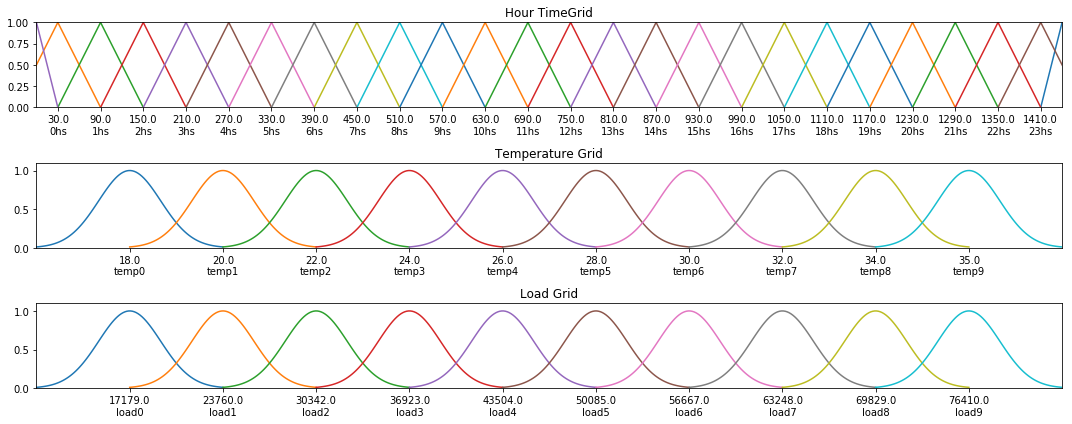
\includegraphics[width=\textwidth]{figures/variables_malaysia.png}
\end{frame}

\note[itemize]{
\item This figure shows an example of the variable set, in this case using the Malaysia Load dataset
}

%%%%%%%%%%%%%%%%%%%%%%%%%%%%%%%%%%%%%%%%%%%%%%
\begin{frame}{$\FIG$-FTS}
\linespread{2}
\begin{itemize}
    \item Each $\vari \in \var$ has its own $\mlvar$, and its own $k_i$,$\mu_i$, $\alpha_i$
    \item Wrapper model which enables a monovariate model (PWFTS) to tackle multivariate time series
    \item $\FIG$-FTS replaces the Partitioning and Fuzzyfication stages of PWFTS
\end{itemize}
\end{frame}

\note[itemize]{
    \item We propose a model that minimally changes the Original PWFTS while enables it to tackle multivariate time series
}




%%%%%%%%%%%%%%%%%%%%%%%%%%%%%%%%%%%%%%%%%%%%%%
\begin{frame}{Fuzzy Information Granules - FIG}
\begin{itemize}
    \item Each FIG $\figi$ is a multivariate fuzzy set
    $$\figi = \{ \mfset \},\qquad \forall \vari \in \var$$
    \item The membership function is the minimum S-Norm
    $$\mu_{\figi} = \bigcap \mu_{\mfset}$$
    \item $\FIG$ is the global linguistic variable, such that $\figi \in \FIG$
\end{itemize}
\end{frame}

\note[itemize]{
    \item FIG's may be created using clustering or just by combining the fuzzy sets of different variables
    \item The combination of fuzzy set is the approach chosen in this research
    \item Why we chose this approach: because it is fast, easy, scalable, easy to distribute
}


%%%%%%%%%%%%%%%%%%%%%%%%%%%%%%%%%%%%%%%%%%%%%%
\begin{frame}{$\FIG$-FTS}
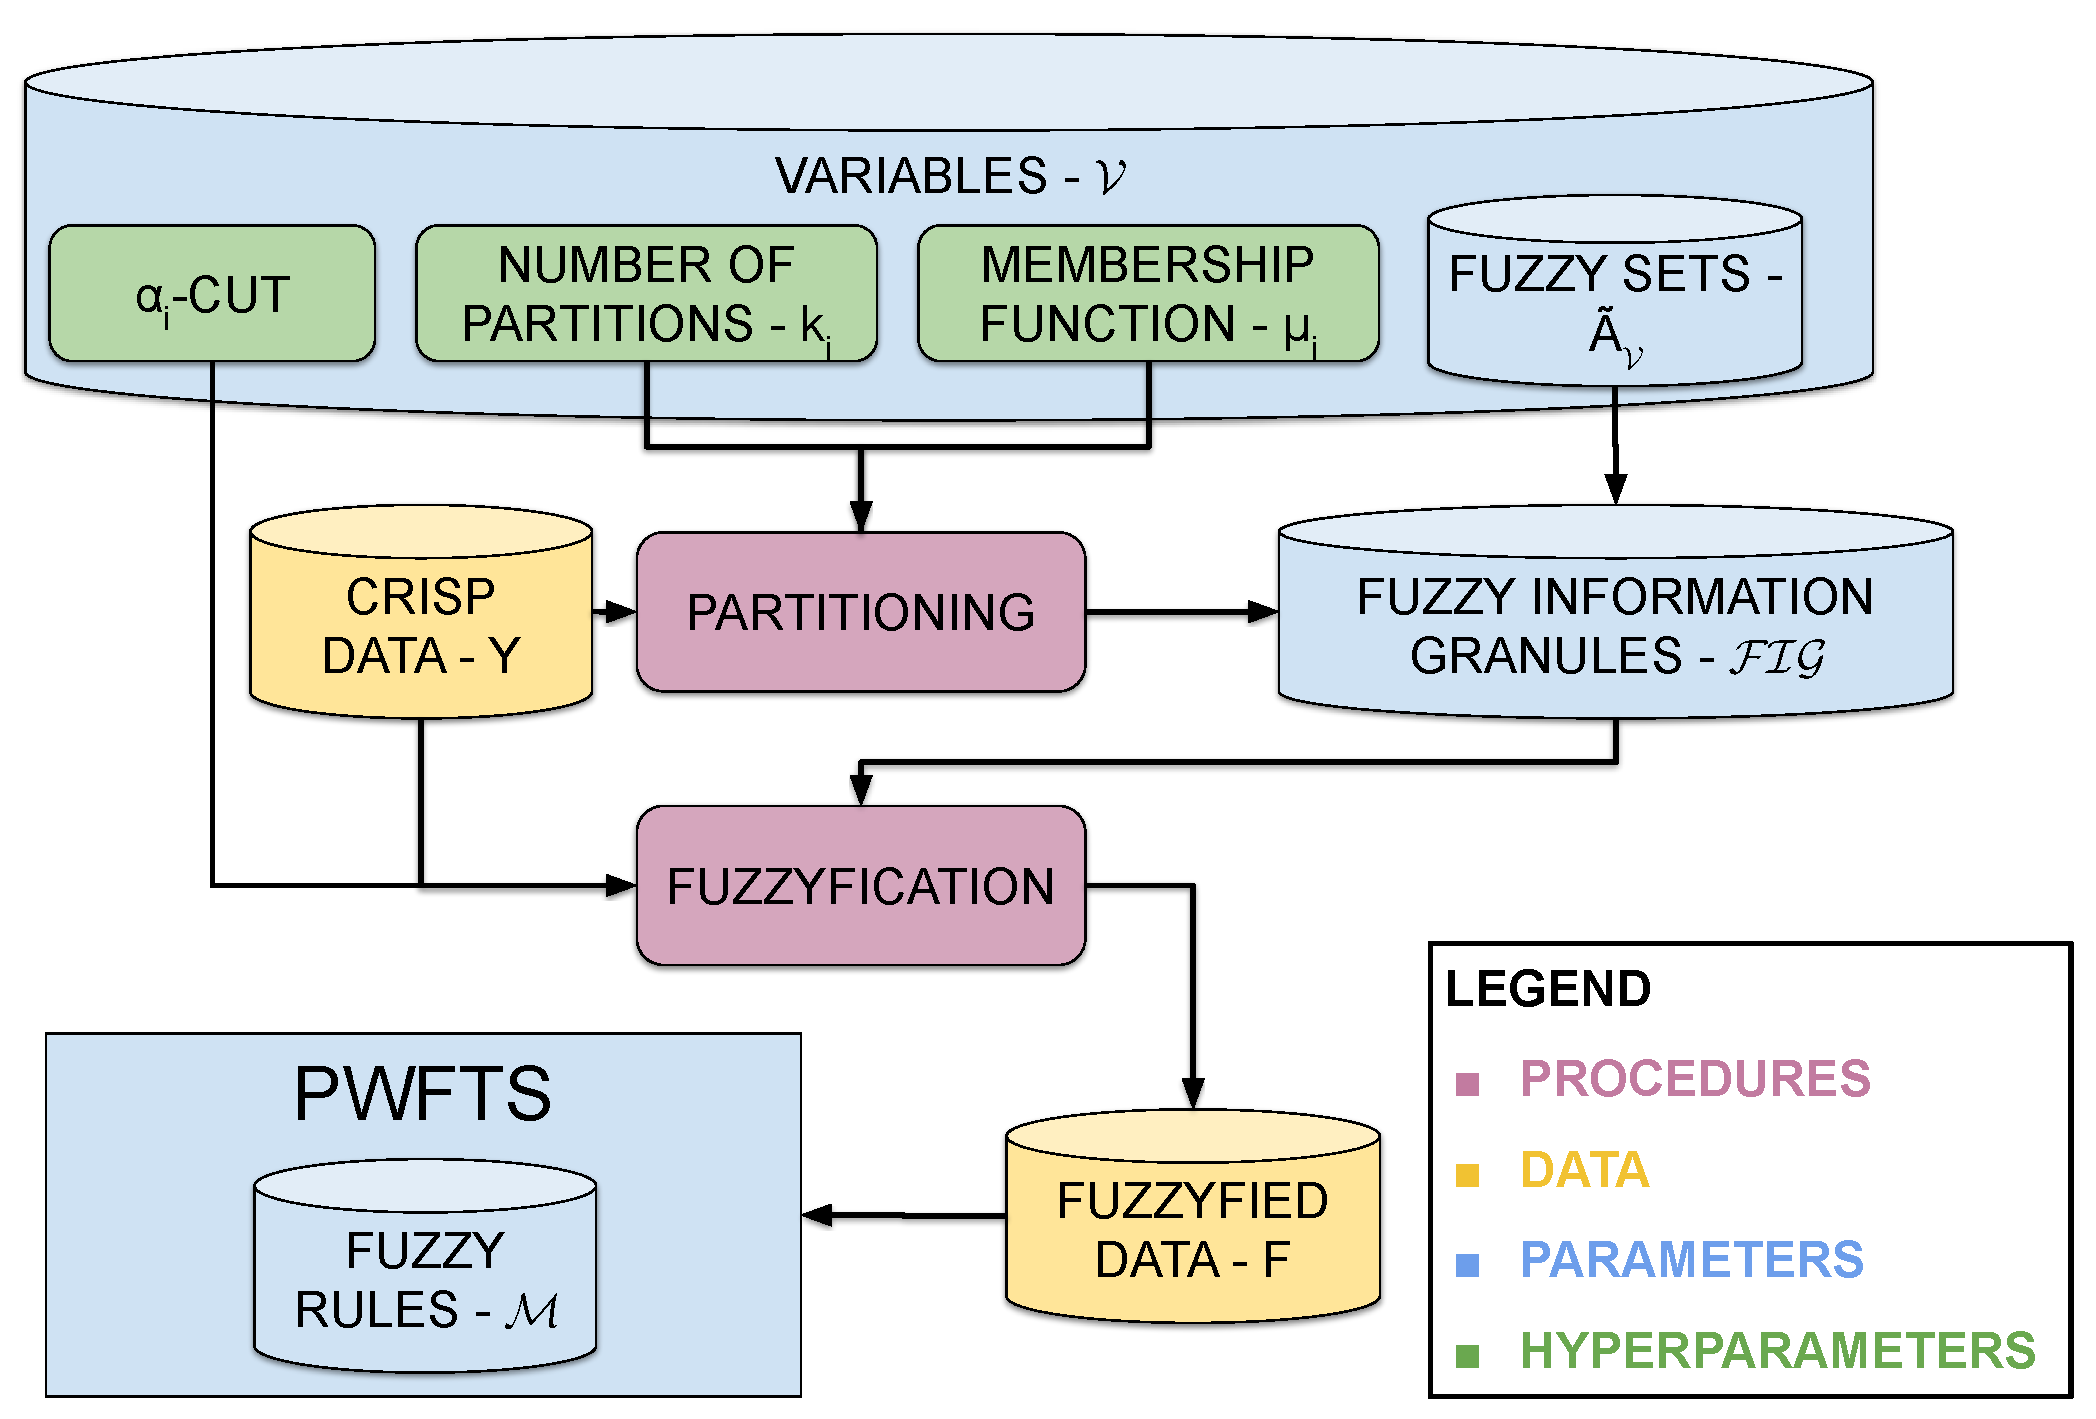
\includegraphics[width=\textwidth]{figures/figfts_training_procedure.pdf}
\end{frame}

%%%%%%%%%%%%%%%%%%%%%%%%%%%%%%%%%%%%%%%%%%%%%%
\begin{frame}{$\FIG$-FTS}
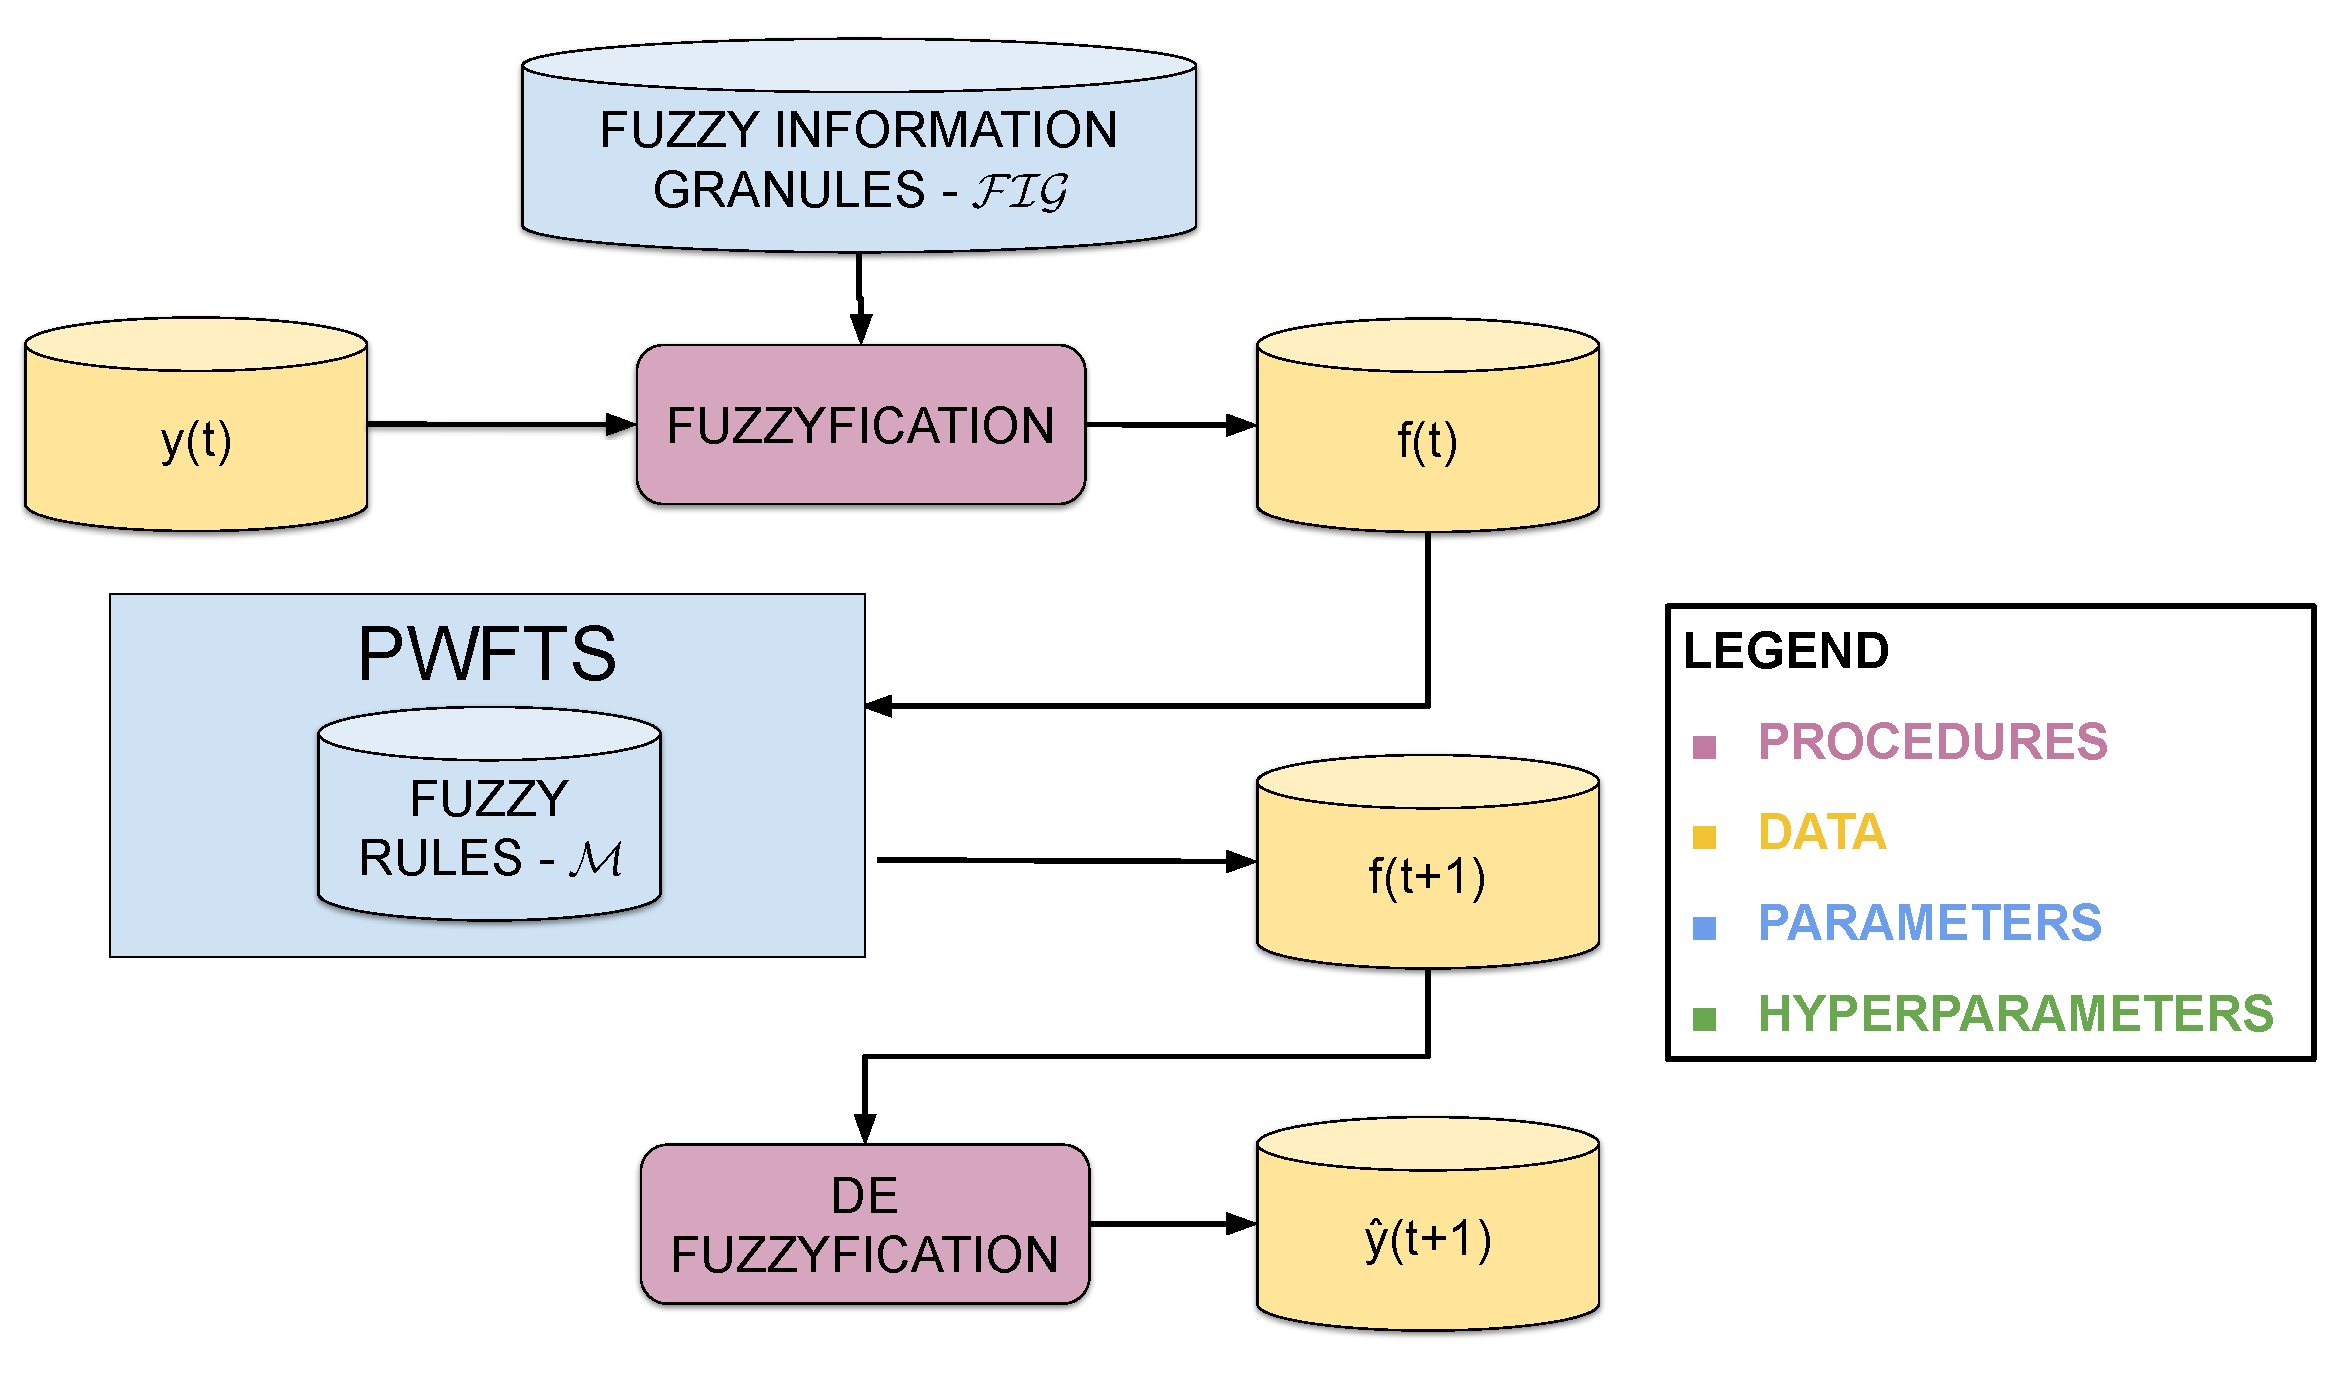
\includegraphics[width=\textwidth]{figures/figfts_forecasting_procedure.pdf}
\end{frame}

%%%%%%%%%%%%%%%%%%%%%%%%%%%%%%%%%%%%%%%%%%%%%%
\begin{frame}{$\FIG$-FTS}
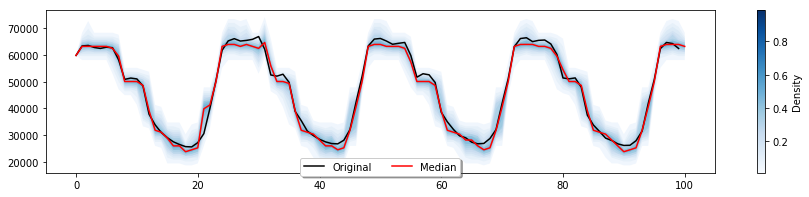
\includegraphics[width=\textwidth,height=6cm]{figures/figfts_probabilistic_onestep.png}
\end{frame}

%%%%%%%%%%%%%%%%%%%%%%%%%%%%%%%%%%%%%%%%%%%%%%
%%%%%%%%%%%%%%%%%%%%%%%%%%%%%%%%%%%%%%%%%%%%%%
\section{Conclusions}

\note[itemize]{
\item Many achievements developed since 2015 were taken out of the thesis due to scope restrictions
\item Many results of the thesis were taken out of this presentation due to time restrictions
\item I invite all of you to read the thesis and also keep following the research results
}

%%%%%%%%%%%%%%%%%%%%%%%%%%%%%%%%%%%%%%%%%%%%%%
\begin{frame}{Main Contributions}
\linespread{2}
\begin{itemize}
    \item First interval forecasting approaches for FTS: $\ifts$, $W\ifts$, Ensemble FTS, PWFTS, $\FIG$-FTS;
    \item First probabilistic forecasting approaches for FTS methods:  Ensemble FTS, PWFTS and $\FIG$-FTS; 
    \item The PWFTS method, an high-order integrated method capable to produce point, interval and probabilistic forecasts for one and many steps ahead, with a white-box model;
\end{itemize}
\end{frame}

\note[itemize]{
\item 
}

%%%%%%%%%%%%%%%%%%%%%%%%%%%%%%%%%%%%%%%%%%%%%%
\begin{frame}{Main Contributions}
\linespread{2}
\begin{itemize}
    \item Scalability approaches based in distributed computing;
    \item Distributed Evolutionary Hyperparameter Optimization (DEHO);
    \item $\FIG$-FTS, an extension of PWFTS for multivariate data. 
\end{itemize}
\end{frame}

\note[itemize]{
\item Once PWFTS was proposed we improve its feature sets with scalability, hyperparam opt and multivariate forecasting 
}

%%%%%%%%%%%%%%%%%%%%%%%%%%%%%%%%%%%%%%%%%%%%%%
\begin{frame}{Limitations}
\linespread{2}
\begin{itemize}
    \item Trend and non-stationarity issues;
    \item Outlier detection;
    \item Hyperparameter tunning of $\FIG$-FTS
\end{itemize}
\end{frame}


%%%%%%%%%%%%%%%%%%%%%%%%%%%%%%%%%%%%%%%%%%%%%%
\begin{frame}{Publications - Journal Papers}
\begin{enumerate}
    \item SILVA, Petrônio C. L.; SADAEI, Hossein J. ; BALLINI, Rosângela ; GUIMARÃES, Frederico G. . Probabilistic Forecasting With Fuzzy Time Series. IEEE Transactions on Fuzzy Systems, v. 1, p. 1-1, 2019. DOI: 10.1109/tfuzz.2019.2922152
    \item SADAEI, Hossein J.; SILVA, Petrônio C. L.; GUIMARÃES, Frederico G.; LEE, Muhammad H. Short-term load forecasting by using a combined method of convolutional neural networks and fuzzy time series. ENERGY, v. 174, p. 1, 2019. DOI: 10.1016/j.energy.2019.03.081
\end{enumerate}
\end{frame}

%%%%%%%%%%%%%%%%%%%%%%%%%%%%%%%%%%%%%%%%%%%%%%
\begin{frame}{Publications - Conference Proceedings}
\scriptsize
\begin{enumerate}
\item  ALVES, M. A.; ALMEIDA, L. V. V. B.; REZENDE, T. M.; SILVA, P. C. L. S.; SEVERIANO, C. A.; SILVA, R.; GUIMARÃES, F. G. Otimização Dinâmica Evolucionária para Despacho de Energia em uma Microrrede usando Veículos Elétricos. In 14º Simpósio Brasileiro de Automação Inteligente - SBAI'19, Ouro Preto, 2019.
\item  LUCAS, P. O. E.; SILVA, P. C. L. S.; GUIMARÃES, F. G. Otimização Evolutiva de Hiperparâmetros para Modelos de Séries Temporais Nebulosas.  In 14º Simpósio Brasileiro de Automação Inteligente - SBAI'19, Ouro Preto, 2019.
\item SILVA, Petrônio C. L.; SEVERIANO Jr., Carlos A.; ALVES, Marcos A. ; COHEN, Miri W.; GUIMARÃES, Frederico G. A New Granular Approach for Multivariate Forecasting. 2nd Latin American Workshop on Computational Neuroscience. Communications in Computer and Information Science, 2019.
\item SILVA, Petrônio C. L.; LUCAS, Patrícia O. ; GUIMARÃES, Frederico G. A Distributed Algorithm for Scalable Fuzzy Time Series. Lecture Notes in Computer Science. 1ed.: Springer International Publishing, 2019, v. , p. 42-56. DOI: 10.1007/978-3-030-19223-5\_4
\end{enumerate}
\end{frame}

%%%%%%%%%%%%%%%%%%%%%%%%%%%%%%%%%%%%%%%%%%%%%%
\begin{frame}{Publications - Conference Proceedings}
\scriptsize
\begin{enumerate}
\item ALVES, Marcos A. ; SILVA, Petrônio C. L. ; SEVERIANO JR., Carlos A. ; VIEIRA, Gustavo L. ; GUIMARAES, Frederico G. ; SADAEI, Hossein J. . An extension of nonstationary fuzzy sets to heteroskedastic fuzzy time series. In: 26th European Symposium on Artificial Neural Networks, Computational Intelligence and Machine Learning, 2018, Bruges, Bélgica. 26th European Symposium on Artificial Neural Networks, Computational Intelligence and Machine Learning, 2018.
\item SILVA, Petrônio C. L.; ALVES, Marcos A. ; SEVERIANO JR., Carlos A. ; VIEIRA, Gustavo L. ; GUIMARAES, Frederido G. ; SADAEI, Hossein J. . Probabilistic Forecasting with Seasonal Ensemble Fuzzy Time-Series. In: XIII Brazilian Congress on Computational Intelligence, 2017, Niterói. Anais do XIII Brazilian Congress on Computational Intelligence, 2017.
\item SEVERIANO Jr, Carlos A.; SILVA, Petrônio C.; SADAEI, Hossein J.; GUIMARÃES, Frederico G. Very Short-term Solar Forecasting using Fuzzy Time Series. 2017 IEEE Conference on Fuzzy Systems. DOI: 10.1109/fuzz-ieee.2017.8015732
\item SILVA, Petrônio C. L.; SADAEI, Hossein J.; GUIMARÃES, Frederico G. Interval Forecasting with Fuzzy Time Series. In Computational Intelligence (SSCI), 2016 IEEE Symposium Series on (pp. 1-8). IEEE. DOI: 10.1109/ssci.2016.7850010
\end{enumerate}
\end{frame}

%%%%%%%%%%%%%%%%%%%%%%%%%%%%%%%%%%%%%%%%%%%%%%
\begin{frame}{Publications}
\begin{itemize}
    \item Short Courses and Talks
    \begin{itemize}
    \item SILVA, Petrônio C. L.; GUIMARÃES, Frederico G. Séries Temporais Nebulosas (STN). In 14º Simpósio Brasileiro de Automação Inteligente - SBAI'19, Ouro Preto, 2019.
    \item SILVA, Petrônio C. L.; GUIMARÃES, Frederico G. Fuzzy Time Series. In pyDATA BH, Belo Horizonte, 2019.
    \item SILVA, Petrônio C. L.; GUIMARÃES, Frederico G. pyFTS Quick Start. In Avenue Code Meetup, Belo Horizonte, 2019.
    \item SILVA, Petrônio C. L.; GUIMARÃES, Frederico G. Introdução às Séries Temporais Nebulosas com Aplicações em Energia Solar. In 2$^a$ Semana de Informática do IFNMG Campus Pirapora, Pirapora, 2018.
\end{itemize}
\end{itemize}
\end{frame}

%%%%%%%%%%%%%%%%%%%%%%%%%%%%%%%%%%%%%%%%%%%%%%
\begin{frame}{Publications}
\begin{itemize}
    \item Computational Libraries
    \begin{itemize}
    \item Silva, P. C. L, et al. pyFTS: Fuzzy Time Series for Python. Source Code: \url{http://pyfts.github.io/pyFTS} DOI: 10.5281/zenodo.597359.
    \end{itemize}
\end{itemize}


\includegraphics[width=\textwidth]{figures/pyfts_logo.png}

\end{frame}

%%%%%%%%%%%%%%%%%%%%%%%%%%%%%%%%%%%%%%%%%%%%%%
\begin{frame}{Publications}
\begin{itemize}
    \item Computational Libraries
    \begin{itemize}
    \item Silva, P. C. L, et al. pyFTS: Fuzzy Time Series for Python. Source Code: \url{http://pyfts.github.io/pyFTS} DOI: 10.5281/zenodo.597359.
    \end{itemize}
\end{itemize}


\includegraphics[width=\textwidth]{figures/pyfts_logo.png}

\end{frame}

%%%%%%%%%%%%%%%%%%%%%%%%%%%%%%%%%%%%%%%%%%%%%%
\begin{frame}{Publications}
\begin{columns}
\column{0.5\textwidth}
\centering
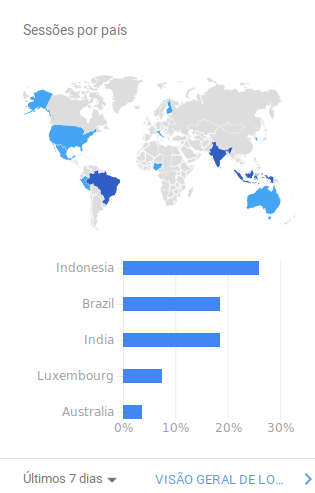
\includegraphics[width=.5\textwidth]{figures/pyfts_last07days.png}
\column{0.5\textwidth}
\centering
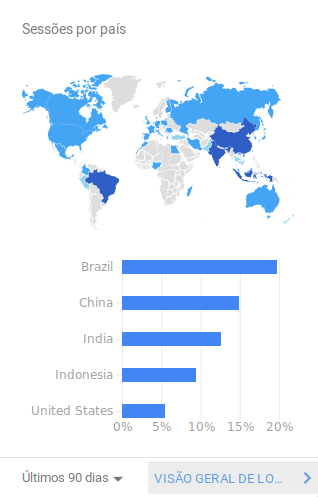
\includegraphics[width=.5\textwidth]{figures/pyfts_last90days.png}
\end{columns}


\end{frame}



%%%%%%%%%%%%%%%%%%%%%%%%%%%%%%%%%%%%%%%%%%%%%%
\begin{frame}{Future Research Directions}
\linespread{2}
\begin{itemize}
    \item Time Variant Models
    \item Hyperparameter optimization for $\FIG$-FTS
    \item Bayesian approach for PWFTS
    \item Joint probability distributions for  $\FIG$-FTS
\end{itemize}
\end{frame}



%%%%%%%%%%%%%%%%%%%%%%%%%%%%%%%%%%%%%%%%%%%%%%
%%%%%%%%%%%%%%%%%%%%%%%%%%%%%%%%%%%%%%%%%%%%%%
\section{References}

\bibliographystyle{apalike}
\bibliography{references}

\end{document}
